\documentclass[10pt,english,aspectratio=169]{beamer}

\usepackage{ae,aecompl}
\usepackage[T1]{fontenc}
\usepackage{textcomp}
\usepackage[utf8]{inputenc}
\usepackage{babel}

\setcounter{secnumdepth}{3}
\setcounter{tocdepth}{3}

\usepackage{amsmath, amssymb, graphicx}
\usepackage{booktabs, multirow}
\usepackage{tikz}
\usetikzlibrary{positioning,arrows.meta,shapes,calc,fit,backgrounds}
\usepackage{listings}
\usepackage{xcolor}
\usepackage{tcolorbox}

\lstset{
  basicstyle=\ttfamily\small,
  keywordstyle=\color{blue!80!black}\bfseries,
  commentstyle=\color{green!50!black}\itshape,
  stringstyle=\color{orange!80!black},
  backgroundcolor=\color{gray!8},
  frame=single,
  rulecolor=\color{gray!40},
  breaklines=true,
  showstringspaces=false,
  numbers=none,
}

\lstdefinestyle{pythonstyle}{
    language=Python,
    basicstyle=\ttfamily\footnotesize,
    keywordstyle=\color{blue!80!black}\bfseries,
    commentstyle=\color{green!50!black}\itshape,
    stringstyle=\color{orange!80!black},
    frame=single,
    rulecolor=\color{gray!40},
    backgroundcolor=\color{gray!8},
    breaklines=true,
    showstringspaces=false,
    numbers=left,
    numbersep=5pt,
    numberstyle=\tiny\color{gray}
}

\lstdefinestyle{yamlstyle}{
    basicstyle=\ttfamily\footnotesize,
    keywordstyle=\color{blue!80!black}\bfseries,
    commentstyle=\color{green!50!black}\itshape,
    stringstyle=\color{orange!80!black},
    frame=single,
    rulecolor=\color{gray!40},
    backgroundcolor=\color{gray!8},
    breaklines=true,
    showstringspaces=false,
    numbers=none,
}

\lstdefinestyle{markdownstyle}{
    basicstyle=\ttfamily\footnotesize,
    frame=single,
    rulecolor=\color{gray!40},
    backgroundcolor=\color{gray!8},
    breaklines=true,
    showstringspaces=false,
    numbers=none,
}

\lstdefinestyle{bashstyle}{
    language=bash,
    basicstyle=\ttfamily\footnotesize,
    keywordstyle=\color{blue!80!black}\bfseries,
    commentstyle=\color{green!50!black}\itshape,
    stringstyle=\color{orange!80!black},
    frame=single,
    rulecolor=\color{gray!40},
    backgroundcolor=\color{gray!8},
    breaklines=true,
    showstringspaces=false,
    numbers=none,
}

\ifx\hypersetup\undefined
  \AtBeginDocument{%
    \hypersetup{bookmarks=false,breaklinks=true,pdfborder={0 0 0},colorlinks=true,
      linkcolor=DarkText,urlcolor=RedTitle}%
  }
\else
  \hypersetup{bookmarks=false,breaklinks=true,pdfborder={0 0 0},colorlinks=true,
    linkcolor=DarkText,urlcolor=RedTitle}%
\fi

\makeatletter
\newcommand\makebeamertitle{\frame{\maketitle}}%
\AtBeginDocument{%
  \let\origtableofcontents=\tableofcontents
  \def\tableofcontents{\@ifnextchar[{\origtableofcontents}{\gobbletableofcontents}}
  \def\gobbletableofcontents#1{\origtableofcontents}%
}

\usetheme{metropolis}
\usefonttheme{professionalfonts}

\definecolor{LightGray}{RGB}{230,230,230}
\definecolor{RedTitle}{RGB}{0,0,200}
\definecolor{VeryLightGray}{RGB}{245,245,245}
\definecolor{DarkText}{RGB}{0,0,0}

\setbeamercolor{background canvas}{bg=white}
\setbeamercolor{title}{fg=RedTitle}
\setbeamercolor{author}{fg=DarkText}
\setbeamercolor{date}{fg=DarkText}
\setbeamercolor{frametitle}{bg=VeryLightGray,fg=DarkText}
\setbeamercolor{normal text}{fg=DarkText}

\setbeamersize{text margin left=5mm, text margin right=5mm}
\addtobeamertemplate{frametitle}{}{\vspace{-0.5em}}
\newcommand{\reducevspace}{\vspace{-0.5cm}}

\setbeamertemplate{navigation symbols}{}
\setbeamertemplate{footline}{%
  \hfill%
  \usebeamercolor[fg]{page number in head/foot}%
  \usebeamerfont{page number in head/foot}%
  \insertframenumber\,/\,\inserttotalframenumber\kern1em\vskip2pt%
}

\makeatother

\graphicspath{{figures/}}


\title[ML \& Agentic AI for Macro Research]{Machine Learning and Agentic AI for Macroeconomic Research\\
10: Case Studies --- Agentic AI in Economic Research\\[0.5em]}
\author{Zhigang Feng}
\date{Spring 2026}

\begin{document}

\makebeamertitle

%===========================================================
% AGENDA
%===========================================================

\begin{frame}{Lecture Agenda}

\begin{columns}[T]
\begin{column}{0.48\textwidth}
\textbf{Part I: Foundations}
\begin{enumerate}
    \item Why case studies?
    \item The research workflow arc
    \item Connecting Lec09 concepts
\end{enumerate}

\vspace{0.3cm}
\textbf{Part II: Case Study 1}\\
\textit{Building a Paper Review Skill}
\begin{enumerate}
  \setcounter{enumi}{3}
    \item The problem \& naive baseline
    \item Skill architecture
    \item Prompt engineering
    \item Running and output
\end{enumerate}
\end{column}

\begin{column}{0.48\textwidth}
\textbf{Part III: Case Study 2}\\
\textit{MEPS Uninsurance Analysis}
\begin{enumerate}
  \setcounter{enumi}{7}
    \item The problem \& naive baseline
    \item Data architecture
    \item Visualization and insights
\end{enumerate}

\vspace{0.3cm}
\textbf{Part IV: Synthesis}
\begin{enumerate}
  \setcounter{enumi}{10}
    \item Lessons and patterns
    \item Lab: MEPS data analysis
\end{enumerate}
\end{column}
\end{columns}

\end{frame}

%===========================================================
\begin{frame}{Where We Are in the Course}

\begin{center}
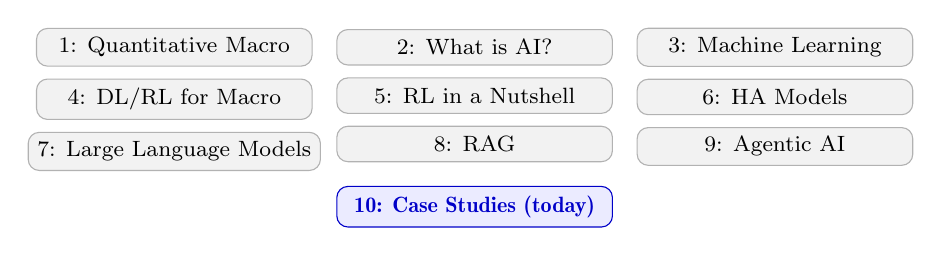
\begin{tikzpicture}[
    node distance=0.25cm,
    lecture/.style={rectangle, rounded corners, draw=gray!60, fill=gray!10,
        minimum width=3.5cm, minimum height=0.45cm, font=\footnotesize, text=DarkText},
    current/.style={rectangle, rounded corners, draw=RedTitle, fill=blue!8,
        minimum width=3.5cm, minimum height=0.45cm, font=\footnotesize\bfseries, text=RedTitle},
]
\node[lecture] (l1) {1: Quantitative Macro};
\node[lecture, right=0.3cm of l1] (l2) {2: What is AI?};
\node[lecture, right=0.3cm of l2] (l3) {3: Machine Learning};

\node[lecture, below=0.15cm of l1] (l4) {4: DL/RL for Macro};
\node[lecture, below=0.15cm of l2] (l5) {5: RL in a Nutshell};
\node[lecture, below=0.15cm of l3] (l6) {6: HA Models};

\node[lecture, below=0.15cm of l4] (l7) {7: Large Language Models};
\node[lecture, below=0.15cm of l5] (l8) {8: RAG};
\node[lecture, below=0.15cm of l6] (l9) {9: Agentic AI};

\node[current, below=0.3cm of l8] (l10) {10: Case Studies (today)};
\end{tikzpicture}
\end{center}

\vspace{0.3cm}
\textbf{The progression:}
\begin{itemize}
    \item Lectures 1--6: Understanding models and AI/ML methods for solving them
    \item Lectures 7--8: Understanding the language model revolution (LLM + RAG)
    \item Lecture 9: Understanding agentic AI tools (skills, agents, sub-agents)
    \item \textbf{Lecture 10: Putting it all together} --- two complete research workflows
\end{itemize}

\end{frame}


%===========================================================
% SECTION: WHY CASE STUDIES?
%===========================================================
\section{Why Case Studies?}

%-----------------------------------------------------------
\begin{frame}{The Gap Between Tools and Research}

\textbf{Lecture 9} gave you the vocabulary: skills, agents, sub-agents, \texttt{CLAUDE.md}, harness engineering, the 5-pillar workflow.

\vspace{0.3cm}
\textbf{But knowing the tools $\neq$ knowing how to use them for research.}

\vspace{0.3cm}
The hard part is \emph{design}:
\begin{itemize}
    \item How do you decompose a research task into agent-sized steps?
    \item How do you encode domain knowledge into prompts?
    \item How do you validate AI-generated output?
    \item When does the agent save time vs.\ create new problems?
\end{itemize}

\vspace{0.3cm}
\textbf{Today: two complete case studies that answer these questions.}
\begin{enumerate}
    \item \textbf{Case Study 1}: Automating academic paper review (NLP + domain expertise)
    \item \textbf{Case Study 2}: Assembling a 25-year panel from MEPS data (data + visualization)
\end{enumerate}

\end{frame}

%-----------------------------------------------------------
\begin{frame}{The Research Workflow Arc}

Both case studies follow the same five-stage arc, adapted from Goldsmith-Pinkham (2026):

\vspace{0.4cm}
\begin{center}
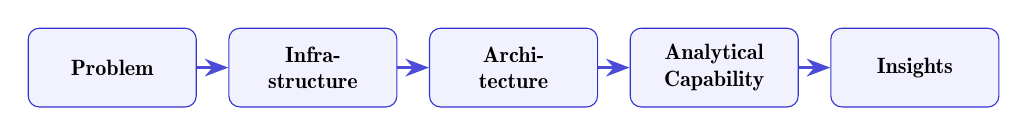
\begin{tikzpicture}[
    stage/.style={rectangle, rounded corners=4pt, draw=RedTitle!80, fill=blue!5,
        minimum width=2.1cm, minimum height=1.0cm, font=\footnotesize\bfseries,
        text width=1.9cm, align=center, text=DarkText},
    arr/.style={-{Stealth[length=3mm]}, thick, RedTitle!70},
]
\node[stage] (p) {Problem};
\node[stage, right=0.4cm of p] (i) {Infra-\\structure};
\node[stage, right=0.4cm of i] (a) {Archi-\\tecture};
\node[stage, right=0.4cm of a] (c) {Analytical\\Capability};
\node[stage, right=0.4cm of c] (o) {Insights};

\draw[arr] (p) -- (i);
\draw[arr] (i) -- (a);
\draw[arr] (a) -- (c);
\draw[arr] (c) -- (o);
\end{tikzpicture}
\end{center}

\vspace{0.3cm}
\begin{small}
\begin{tabular}{lll}
\toprule
\textbf{Stage} & \textbf{Case Study 1 (Paper Review)} & \textbf{Case Study 2 (MEPS Data)} \\
\midrule
Problem & Reviewing papers is hard & 24 years of survey data \\
Infrastructure & Skill folder + YAML config & Claude Code + Python env \\
Architecture & 7-phase review pipeline & Download $\to$ Harmonize $\to$ Analyze \\
Capability & Prompt engineering + filters & Weighted statistics by group \\
Insights & Structured referee report & 6 publication-quality figures \\
\bottomrule
\end{tabular}
\end{small}

\vspace{0.2cm}
{\footnotesize Reference: Paul Goldsmith-Pinkham, ``Large Datasets and Structured Databases: Claude Code for Economists,'' 2026.}

\end{frame}

%-----------------------------------------------------------
\begin{frame}{What Lec09 Concepts Recur Today}

\begin{small}
\begin{tabular}{p{3.5cm}p{5.0cm}p{4.5cm}}
\toprule
\textbf{Lec09 Concept} & \textbf{Case Study 1 (Paper Review)} & \textbf{Case Study 2 (MEPS Data)} \\
\midrule
\textbf{Skills} & The entire review-paper skill & Ad hoc prompts (no skill needed) \\
\textbf{Agents / sub-agents} & 3 calibration agents, $N$ section reviewers & Single-session workflow \\
\textbf{Shared directives} & \texttt{shared-directives.md} (tone, confidence) & \texttt{CLAUDE.md} (project context) \\
\textbf{Iterative workflow} & Edit prompt $\to$ rerun $\to$ inspect & Prompt $\to$ inspect $\to$ refine \\
\textbf{Pillar 5 (Verify)} & Check math claims, judge domain fit & Cross-check vs.\ Census Bureau \\
\bottomrule
\end{tabular}
\end{small}

\vspace{0.4cm}
\textbf{Key observation:} Case Study 1 is a \emph{skill} (reusable, multi-phase, quality-gated).\\
Case Study 2 is \emph{ad hoc} (one-off, 3 prompts, single session).

\vspace{0.2cm}
Both are legitimate. The choice depends on: \emph{How often will you do this? How much quality control do you need?}

\end{frame}


%===========================================================
% SECTION: CASE STUDY 1 --- THE PROBLEM
%===========================================================
\section{Case Study 1: The Problem}

%-----------------------------------------------------------
\begin{frame}{The Naive Baseline: Paste a Paper into ChatGPT}

\textbf{The tempting approach:} Copy your paper's abstract into ChatGPT and ask ``review this paper.''

\vspace{0.3cm}
\textbf{What you get:}
\begin{itemize}
    \item Generic praise: \textit{``The paper makes an important contribution to the literature\ldots''}
    \item Surface-level suggestions: \textit{``The authors should discuss limitations\ldots''}
    \item No verbatim quotes from the paper
    \item No equation verification
    \item No domain-calibrated assessment
\end{itemize}

\vspace{0.3cm}
\textbf{What's missing:}
\begin{enumerate}
    \item No extraction pipeline --- the LLM sees a wall of text, not structured sections
    \item No domain calibration --- it doesn't know what matters in quantitative macro
    \item No specialization --- proofs need different attention than methodology
    \item No quality gate --- hallucinated comments survive unchecked
    \item No quote verification --- it may ``quote'' text the paper never said
\end{enumerate}

\end{frame}

%-----------------------------------------------------------
\begin{frame}[fragile]{What a Good Referee Report Looks Like}

A structured review has clear components:

\vspace{0.2cm}
\begin{tcolorbox}[colback=gray!5, colframe=gray!40, title={\footnotesize Example: refine.ink output format}, fonttitle=\bfseries\footnotesize]
\begin{lstlisting}[style=markdownstyle, basicstyle=\ttfamily\scriptsize]
# Regression Discontinuity Design with Distribution

**Date**: 03/03/2026
**Domain**: social_sciences/economics
**Taxonomy**: academic/research_paper

## Overall Feedback
**Estimand definition needs tightening**
The paper defines the estimand as a weighted average
of treatment effects but the weighting function is
never made explicit. In Section 2.3, equation (7)...

## Detailed Comments (20)
### 1. Sign error in Theorem 2 proof
**Quote**: > "By dominated convergence, $\lim_{h\to 0}..."
**Feedback**: The dominated convergence step requires...
\end{lstlisting}
\end{tcolorbox}

\vspace{0.2cm}
\textbf{Properties:} 4--8 overview issues with section/equation references $\cdot$ 8--25 detailed comments with \emph{verbatim quotes} $\cdot$ Severity ratings $\cdot$ Recommendation + revision targets.

\vspace{0.1cm}
This cannot be produced by a single prompt.

\end{frame}

%-----------------------------------------------------------
\begin{frame}{The Paper We Will Review}

\begin{tcolorbox}[colback=blue!3, colframe=RedTitle!60, title={\footnotesize Demo Paper}, fonttitle=\bfseries\footnotesize]
\textbf{Markov Equilibria with Quasi-Hyperbolic Discounting}\\
\textit{Zhigang Feng (University of Nebraska Omaha) and Manuel S.\ Santos (University of Miami)}
\end{tcolorbox}

\vspace{0.2cm}
\textbf{Content:}
\begin{itemize}
    \item Neoclassical growth model with $(\beta, \delta)$ quasi-hyperbolic preferences
    \item Proves existence of Markov equilibria via a sequence of $\varepsilon$-equilibria
    \item Establishes saddle-path stability of steady states (ruling out indeterminacy)
    \item Numerical computation of equilibrium policy functions
\end{itemize}

\vspace{0.2cm}
\textbf{Why this paper is a good test case:}
\begin{enumerate}
    \item \textbf{Proofs} that need step-by-step verification (Theorems on existence, stability)
    \item \textbf{Numerical results} that can be checked for internal consistency
    \item \textbf{Domain-specific methodology} (dynamic programming, Markov equilibrium)
    \item \textbf{Cross-section claims} (discussion section vs.\ formal results)
\end{enumerate}

\end{frame}

%-----------------------------------------------------------
\begin{frame}{What We Want the Skill to Produce}

Given the paper as input, the skill should output:

\vspace{0.3cm}
\begin{columns}[T]
\begin{column}{0.48\textwidth}
\textbf{Overview Assessment}
\begin{itemize}
    \item 4--8 macro-level issues
    \item Each with section/equation references
    \item Concrete remediation suggestions
    \item Recommendation: accept / minor / major / reject
    \item Key revision targets
\end{itemize}
\end{column}

\begin{column}{0.48\textwidth}
\textbf{Detailed Comments}
\begin{itemize}
    \item 8--25 section-level comments
    \item Each anchored to a \textbf{verbatim quote}
    \item Severity: critical / major / minor
    \item Confidence: high / medium / low
    \item Feedback: 3--8 sentences with concrete fix
\end{itemize}
\end{column}
\end{columns}

\vspace{0.4cm}
\textbf{The design challenge:} How do we break this into stages that are each small enough for one agent call, but together cover the full review?

\vspace{0.2cm}
$\Rightarrow$ This is an \textbf{orchestration problem} --- exactly what Claude Code skills are designed for.

\end{frame}

%-----------------------------------------------------------
\begin{frame}{The Design Challenge: Why Decomposition?}

\textbf{Why can't a single prompt do this?}

\vspace{0.3cm}
\begin{enumerate}
    \item \textbf{Context window limits.} A 60-page paper + all review instructions + output format exceeds a single agent call. The skill loads prompts on demand.

    \vspace{0.2cm}
    \item \textbf{Specialization.} Checking a proof step-by-step requires different attention than evaluating whether a methodology section properly identifies its assumptions. Different prompts for different section types.

    \vspace{0.2cm}
    \item \textbf{Quality control.} Without an editorial filter, you get 40 comments --- half generic, half wrong. A dedicated quality gate catches hallucinated quotes and generic advice.
\end{enumerate}

\vspace{0.3cm}
\textbf{The analogy:} You would not ask a single RA to simultaneously extract data, calibrate review criteria, write deep section reviews, and edit the final report. You decompose the task and assign specialized roles.

\vspace{0.2cm}
$\Rightarrow$ The skill decomposes the review into \textbf{7 sequential phases}, with parallelism \emph{within} phases.

\end{frame}


%===========================================================
% SECTION: CASE STUDY 1 --- SKILL ARCHITECTURE
%===========================================================
\section{Case Study 1: Skill Architecture}

%-----------------------------------------------------------
\begin{frame}[fragile]{The File Layout (1/2)}

\begin{columns}[T]
\begin{column}{0.45\textwidth}
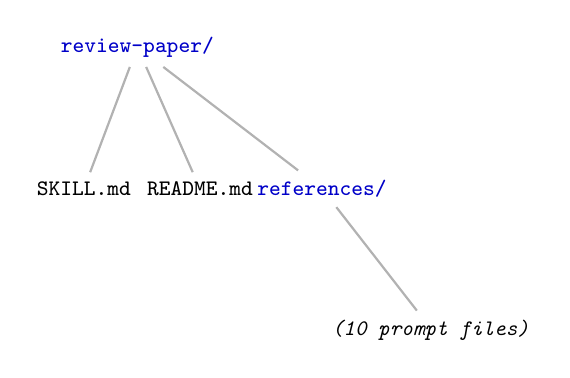
\begin{tikzpicture}[
    every node/.style={font=\ttfamily\footnotesize, anchor=west},
    edge from parent/.style={draw, thick, gray!60},
    level distance=1.8cm,
    sibling distance=1.4cm,
]
\node[font=\ttfamily\footnotesize\bfseries] {\textcolor{RedTitle}{review-paper/}}
    child { node {SKILL.md} }
    child { node {README.md} }
    child { node[font=\ttfamily\footnotesize\bfseries] {\textcolor{RedTitle}{references/}}
        child { node {\textit{(10 prompt files)}} }
    };
\end{tikzpicture}
\end{column}

\begin{column}{0.52\textwidth}
\textbf{Two types of files:}

\vspace{0.2cm}
\textbf{1. The orchestrator} (\texttt{SKILL.md})
\begin{itemize}
    \item Defines the 7-phase pipeline
    \item Tells Claude \emph{which} reference files to read and \emph{when}
    \item Written in plain English
\end{itemize}

\vspace{0.2cm}
\textbf{2. Reference prompts} (\texttt{references/*.md})
\begin{itemize}
    \item Specialized instructions for each phase
    \item Loaded on demand (not all at once)
    \item Each file is self-contained
\end{itemize}

\vspace{0.2cm}
\textbf{Key insight:} The skill is a \emph{folder}, not a single file. Installation is copying a folder.
\end{column}
\end{columns}

\end{frame}

%-----------------------------------------------------------
\begin{frame}[fragile]{The File Layout (2/2)}

\textbf{Inside \texttt{references/}:}

\vspace{0.3cm}
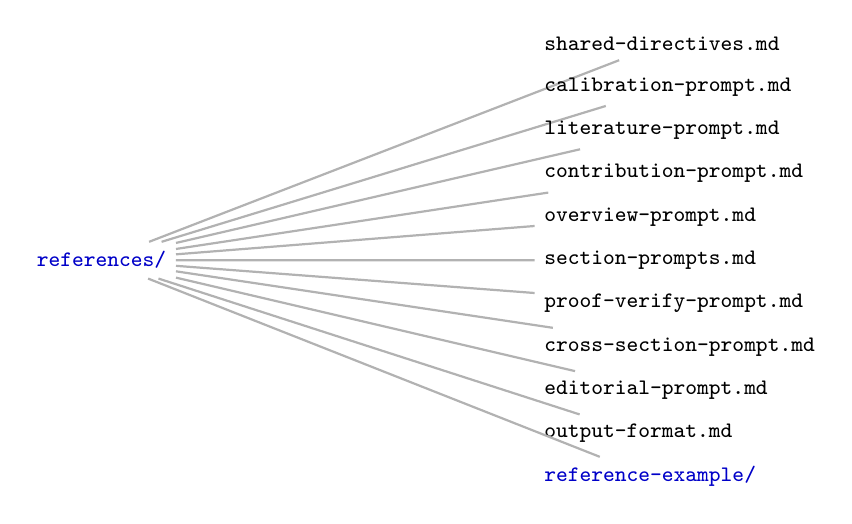
\begin{tikzpicture}[
    every node/.style={font=\ttfamily\footnotesize, anchor=west},
    edge from parent/.style={draw, thick, gray!60},
    grow'=right,
    level distance=5.5cm,
    sibling distance=0.55cm,
]
\node[font=\ttfamily\footnotesize\bfseries] {\textcolor{RedTitle}{references/}}
    child { node {shared-directives.md} }
    child { node {calibration-prompt.md} }
    child { node {literature-prompt.md} }
    child { node {contribution-prompt.md} }
    child { node {overview-prompt.md} }
    child { node {section-prompts.md} }
    child { node {proof-verify-prompt.md} }
    child { node {cross-section-prompt.md} }
    child { node {editorial-prompt.md} }
    child { node {output-format.md} }
    child { node[font=\ttfamily\footnotesize\bfseries] {\textcolor{RedTitle}{reference-example/}} };
\end{tikzpicture}

\vspace{0.3cm}
\small Each file contains \textbf{specialized instructions} loaded on demand --- one phase at a time.

\end{frame}

%-----------------------------------------------------------
\begin{frame}[fragile]{Alternative: The \texttt{.claude/} Project Folder}

\begin{columns}[T]
\begin{column}{0.46\textwidth}
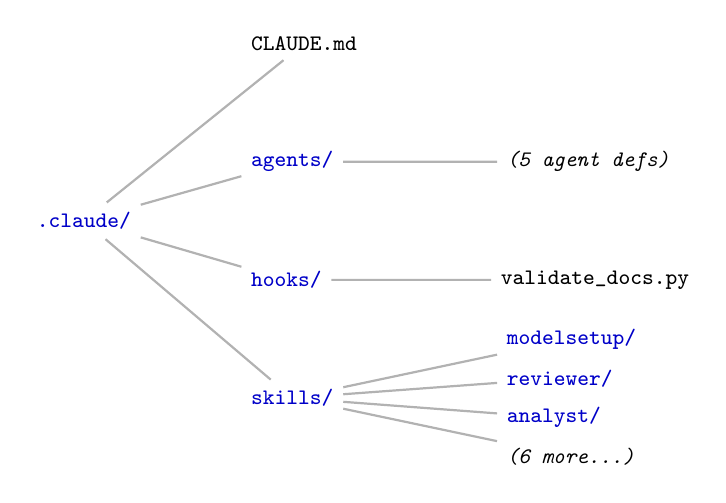
\begin{tikzpicture}[
    every node/.style={font=\ttfamily\footnotesize, anchor=west},
    edge from parent/.style={draw, thick, gray!60},
    grow'=right,
    level 1/.style={sibling distance=1.5cm, level distance=2.0cm},
    level 2/.style={sibling distance=0.5cm,  level distance=2.6cm},
]
\node[font=\ttfamily\footnotesize\bfseries] {\textcolor{RedTitle}{.claude/}}
    child { node {CLAUDE.md} }
    child { node[font=\ttfamily\footnotesize\bfseries] {\textcolor{RedTitle}{agents/}}
        child { node {\textit{(5 agent defs)}} }
    }
    child { node[font=\ttfamily\footnotesize\bfseries] {\textcolor{RedTitle}{hooks/}}
        child { node {validate\_docs.py} }
    }
    child { node[font=\ttfamily\footnotesize\bfseries] {\textcolor{RedTitle}{skills/}}
        child { node {\textcolor{RedTitle}{modelsetup/}} }
        child { node {\textcolor{RedTitle}{reviewer/}} }
        child { node {\textcolor{RedTitle}{analyst/}} }
        child { node {\textit{(6 more\ldots)}} }
    };
\end{tikzpicture}
\end{column}

\begin{column}{0.51\textwidth}
\textbf{Skills live inside \texttt{.claude/}:}

\vspace{0.2cm}
\textbf{\texttt{CLAUDE.md}} --- persistent project memory \& global instructions for Claude

\vspace{0.2cm}
\textbf{\texttt{agents/}} --- subagent persona definitions
\begin{itemize}
    \item Each agent has a specialized role (algorithmist, reviewer, \ldots)
    \item Invoked by the orchestrator during multi-agent tasks
\end{itemize}

\vspace{0.2cm}
\textbf{\texttt{hooks/}} --- event-driven automation
\begin{itemize}
    \item Scripts triggered by Claude Code events
    \item E.g., validate documentation after each edit
\end{itemize}

\vspace{0.2cm}
\textbf{\texttt{skills/}} --- multiple skill folders, same structure as before

\vspace{0.2cm}
\textbf{Key difference:} One \texttt{.claude/} folder manages \emph{all} skills, agents, and automation for a project.
\end{column}
\end{columns}

\end{frame}

%-----------------------------------------------------------
\begin{frame}[fragile]{The YAML Frontmatter}

Every skill starts with YAML frontmatter in \texttt{SKILL.md}:

\vspace{0.2cm}
\begin{lstlisting}[style=yamlstyle]
---
name: review-paper
description: >
  Review an academic paper using the coarse multi-stage
  peer review pipeline. Produces a refine.ink-format
  markdown report with macro-level issues and detailed
  comments with verbatim quotes. Use when the user wants
  to review a paper, get feedback on a manuscript, or
  generate a referee report.
  Triggers on: "review this paper", "peer review",
  "referee report", "/review-paper path/to/paper.pdf".
---
\end{lstlisting}

\vspace{0.2cm}
\begin{itemize}
    \item \texttt{name}: Used for routing --- \texttt{/review-paper} invokes this skill
    \item \texttt{description}: Claude pattern-matches these phrases to decide \emph{when} to invoke the skill automatically
    \item Arguments: \texttt{\$ARGUMENTS} = the path to the paper file (PDF, TeX, etc.)
\end{itemize}

\end{frame}

%-----------------------------------------------------------
\begin{frame}{The 7-Phase Pipeline}

\begin{center}
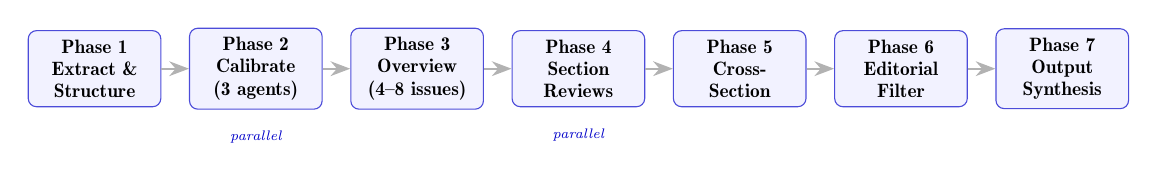
\begin{tikzpicture}[
    phase/.style={rectangle, rounded corners=3pt, draw=RedTitle!70, fill=blue!5,
        minimum width=1.5cm, minimum height=0.85cm, font=\scriptsize\bfseries,
        text width=1.45cm, align=center, text=DarkText},
    arr/.style={-{Stealth[length=2.5mm]}, thick, gray!60},
    parlabel/.style={font=\tiny\itshape, text=RedTitle},
]
\node[phase] (p1) {Phase 1\\Extract \&\\Structure};
\node[phase, right=0.35cm of p1] (p2) {Phase 2\\Calibrate\\(3 agents)};
\node[phase, right=0.35cm of p2] (p3) {Phase 3\\Overview\\(4--8 issues)};
\node[phase, right=0.35cm of p3] (p4) {Phase 4\\Section\\Reviews};
\node[phase, right=0.35cm of p4] (p5) {Phase 5\\Cross-\\Section};
\node[phase, right=0.35cm of p5] (p6) {Phase 6\\Editorial\\Filter};
\node[phase, right=0.35cm of p6] (p7) {Phase 7\\Output\\Synthesis};

\draw[arr] (p1) -- (p2);
\draw[arr] (p2) -- (p3);
\draw[arr] (p3) -- (p4);
\draw[arr] (p4) -- (p5);
\draw[arr] (p5) -- (p6);
\draw[arr] (p6) -- (p7);

% Parallel labels
\node[parlabel, below=0.15cm of p2] {parallel};
\node[parlabel, below=0.15cm of p4] {parallel};
\end{tikzpicture}
\end{center}

\vspace{0.2cm}
\begin{small}
\begin{tabular}{clp{8cm}}
\toprule
\textbf{Phase} & \textbf{Name} & \textbf{What It Does} \\
\midrule
1 & Extract \& Structure & Read paper, parse into sections, classify types, extract claims \\
2 & Calibrate & 3 parallel agents: domain calibration, literature search, contribution extraction \\
3 & Overview & Generate 4--8 macro-level issues + recommendation \\
4 & Section Reviews & Parallel agents with specialized prompts (proof, methodology, results, \ldots) \\
5 & Cross-Section & Check: do discussion claims match formal results? \\
6 & Editorial Filter & 7-step quality gate: dedup, quote verify, severity assign, humanize \\
7 & Output Synthesis & Render final review in refine.ink format \\
\bottomrule
\end{tabular}
\end{small}

\end{frame}

%-----------------------------------------------------------
\begin{frame}{Why 7 Phases, Not 1?}

\textbf{Naive approach:} ``Read this paper and write a comprehensive review.'' (One giant prompt.)

\vspace{0.4cm}
\textbf{Three reasons for decomposition:}

\vspace{0.2cm}
\begin{columns}[T]
\begin{column}{0.32\textwidth}
\textbf{1. Context window}

A 60-page paper + all review instructions + output template exceeds a single call.

The skill loads only the prompts needed for each phase.
\end{column}

\begin{column}{0.32\textwidth}
\textbf{2. Specialization}

Proof-checking requires step-by-step mathematical re-derivation.

Methodology review requires checking identification assumptions.

One prompt cannot do both well.
\end{column}

\begin{column}{0.32\textwidth}
\textbf{3. Quality control}

Without an editorial filter, you get 40 comments --- half are generic advice, some ``quote'' text that doesn't exist.

The filter catches these.
\end{column}
\end{columns}

\vspace{0.4cm}
$\Rightarrow$ \textbf{Parallelism is within phases} (3 calibration agents, $N$ section agents), \textbf{not between phases} (each phase depends on the previous).

\end{frame}

%-----------------------------------------------------------
\begin{frame}{Sequential Dependencies}

\begin{center}
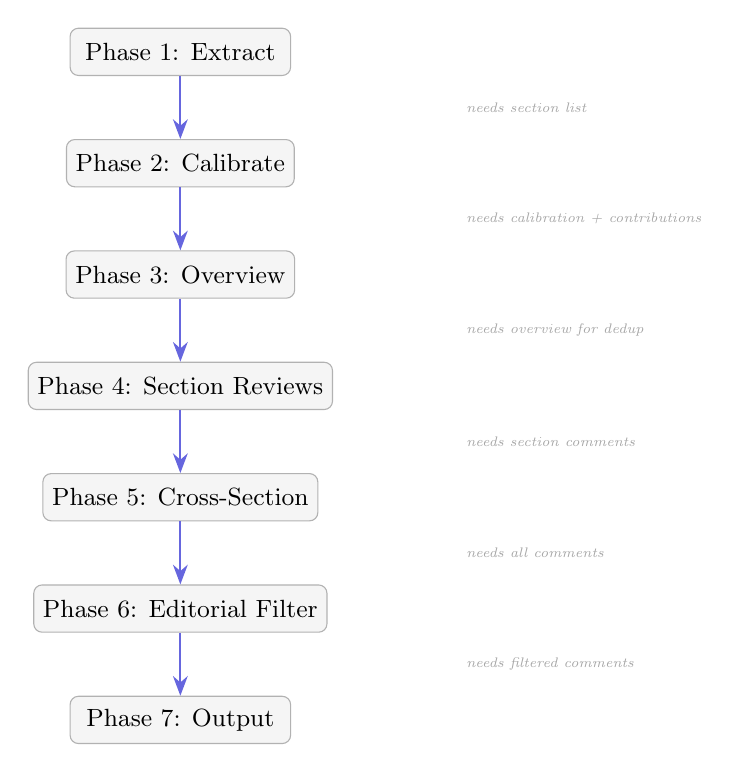
\begin{tikzpicture}[
    node distance=0.8cm,
    phase/.style={rectangle, rounded corners=3pt, draw=gray!60, fill=gray!8,
        minimum width=2.8cm, minimum height=0.6cm, font=\small, text=DarkText},
    dep/.style={-{Stealth[length=2.5mm]}, thick, RedTitle!60},
    reason/.style={font=\tiny\itshape, text=gray!70, anchor=west},
]
\node[phase] (p1) {Phase 1: Extract};
\node[phase, below=of p1] (p2) {Phase 2: Calibrate};
\node[phase, below=of p2] (p3) {Phase 3: Overview};
\node[phase, below=of p3] (p4) {Phase 4: Section Reviews};
\node[phase, below=of p4] (p5) {Phase 5: Cross-Section};
\node[phase, below=of p5] (p6) {Phase 6: Editorial Filter};
\node[phase, below=of p6] (p7) {Phase 7: Output};

\draw[dep] (p1) -- (p2) node[reason, midway, xshift=3.5cm] {needs section list};
\draw[dep] (p2) -- (p3) node[reason, midway, xshift=3.5cm] {needs calibration + contributions};
\draw[dep] (p3) -- (p4) node[reason, midway, xshift=3.5cm] {needs overview for dedup};
\draw[dep] (p4) -- (p5) node[reason, midway, xshift=3.5cm] {needs section comments};
\draw[dep] (p5) -- (p6) node[reason, midway, xshift=3.5cm] {needs all comments};
\draw[dep] (p6) -- (p7) node[reason, midway, xshift=3.5cm] {needs filtered comments};
\end{tikzpicture}
\end{center}

\end{frame}

%-----------------------------------------------------------
\begin{frame}[fragile]{The Orchestrator Pattern in SKILL.md}

The SKILL.md file orchestrates by telling Claude what to read and when. Here is Phase 2:

\vspace{0.2cm}
\begin{lstlisting}[style=markdownstyle, basicstyle=\ttfamily\scriptsize]
## Phase 2: Calibrate (3 Parallel Agents)

Launch 3 agents simultaneously using the Agent tool:

**Agent 1 -- Domain Calibration**
- Read: references/calibration-prompt.md
- Read: references/shared-directives.md
- Input: paper metadata + abstract
- Output: domain-specific review criteria

**Agent 2 -- Literature Search**
- Read: references/literature-prompt.md
- Use WebSearch to find 8-10 related papers
- Output: related work with relevance notes

**Agent 3 -- Contribution Extraction**
- Read: references/contribution-prompt.md
- Input: full paper text
- Output: stated contributions as bullet list

Collect all 3 results before proceeding to Phase 3.
\end{lstlisting}

\vspace{0.1cm}
$\Rightarrow$ Plain English, but precise: \emph{which files} to read, \emph{what} to pass, \emph{when} to wait.

\end{frame}

%-----------------------------------------------------------
\begin{frame}{Reference Files = Specialized Prompts}

\begin{small}
\begin{tabular}{lcp{7.5cm}}
\toprule
\textbf{Reference File} & \textbf{Phase} & \textbf{Role} \\
\midrule
\texttt{shared-directives.md} & All & Tone, confidence gate, quote rules, steelman protocol \\
\texttt{calibration-prompt.md} & 2 & Generate domain-specific review criteria \\
\texttt{literature-prompt.md} & 2 & WebSearch for 8--10 related papers \\
\texttt{contribution-prompt.md} & 2 & Extract the paper's stated contributions \\
\texttt{overview-prompt.md} & 3 & Identify 4--8 macro-level issues + recommendation \\
\texttt{section-prompts.md} & 4 & 6 specialized review variants (proof, methodology, results, literature, discussion, general) \\
\texttt{proof-verify-prompt.md} & 4b & Adversarial two-pass proof verification \\
\texttt{cross-section-prompt.md} & 5 & Check discussion vs.\ formal results alignment \\
\texttt{editorial-prompt.md} & 6 & 7-step quality gate \\
\texttt{output-format.md} & 7 & refine.ink rendering template \\
\bottomrule
\end{tabular}
\end{small}

\vspace{0.3cm}
\textbf{Key design principle:} Each file is self-contained. Only the agents that need a file read it. This keeps each agent's context window efficient.

\end{frame}

%-----------------------------------------------------------
\begin{frame}{Why Reference Files Live Outside SKILL.md}

\textbf{Q:} Why not put all the prompts directly into SKILL.md?

\vspace{0.3cm}
\textbf{A:} Three reasons.

\vspace{0.2cm}
\begin{enumerate}
    \item \textbf{Context efficiency.} The section reviewer only reads \texttt{section-prompts.md} and \texttt{shared-directives.md}. It never sees \texttt{editorial-prompt.md}. If everything were in one file, every agent would load every prompt.

    \vspace{0.2cm}
    \item \textbf{Modularity.} You can improve the editorial filter without touching the section prompts. Each file is independently editable and testable.

    \vspace{0.2cm}
    \item \textbf{Reusability.} \texttt{shared-directives.md} is read by every phase. If it were embedded in SKILL.md, you'd have to duplicate it or use fragile references.
\end{enumerate}

\vspace{0.3cm}
\textbf{Analogy:} A referee coordinator gives each sub-referee a different rubric. The coordinator's job is to assign tasks and collect results --- not to memorize all the rubrics.

\end{frame}


%===========================================================
% SECTION: CASE STUDY 1 --- PROMPT ENGINEERING
%===========================================================
\section{Case Study 1: Prompt Engineering}

%-----------------------------------------------------------
\begin{frame}[fragile]{Shared Directives: The Foundation}

\texttt{shared-directives.md} is injected into \emph{every} review phase. Key excerpts:

\vspace{0.2cm}
\begin{columns}[T]
\begin{column}{0.48\textwidth}
\textbf{Tone}
\begin{lstlisting}[style=markdownstyle, basicstyle=\ttfamily\scriptsize]
Write as a constructive but
direct colleague. Vary phrasing.
Do NOT always start with
"It would be helpful to..."
\end{lstlisting}

\vspace{0.1cm}
\textbf{Banned Vocabulary}
\begin{lstlisting}[style=markdownstyle, basicstyle=\ttfamily\scriptsize]
Never use: crucial, comprehensive,
robust, multifaceted, delve,
landscape, facilitate, holistic,
pivotal, leverages
\end{lstlisting}
\end{column}

\begin{column}{0.48\textwidth}
\textbf{Confidence Gate}
\begin{lstlisting}[style=markdownstyle, basicstyle=\ttfamily\scriptsize]
Only claim an error if you can
support it concretely with a
derivation or citation.
If uncertain, phrase as a question.
\end{lstlisting}

\vspace{0.1cm}
\textbf{Steelman Protocol}
\begin{lstlisting}[style=markdownstyle, basicstyle=\ttfamily\scriptsize]
Before claiming a proof step is
wrong: (1) state what the authors
intended, (2) check their own
defense (remarks, footnotes),
(3) verify conditions are needed.
\end{lstlisting}
\end{column}
\end{columns}

\vspace{0.2cm}
$\Rightarrow$ These directives prevent the most common AI review failures: generic praise, AI-sounding language, hallucinated errors, uncharitable reading.

\end{frame}

%-----------------------------------------------------------
\begin{frame}{Why Humanization Matters}

\textbf{Without} shared directives:

\vspace{0.1cm}
\begin{tcolorbox}[colback=red!3, colframe=red!40, fonttitle=\bfseries\footnotesize, title=AI-sounding review]
{\footnotesize\itshape ``This paper makes a \textbf{crucial} contribution to the \textbf{robust} literature on \textbf{multifaceted} aspects of time-inconsistent preferences. The authors \textbf{delve} into the \textbf{landscape} of Markov equilibria\ldots''}
\end{tcolorbox}

\vspace{0.2cm}
\textbf{With} shared directives:

\vspace{0.1cm}
\begin{tcolorbox}[colback=green!3, colframe=green!40, fonttitle=\bfseries\footnotesize, title=Human-sounding review]
{\footnotesize\itshape ``The paper proves existence of Markov equilibria via $\varepsilon$-equilibria. The construction circumvents the non-removable discontinuities in the equilibrium mapping, which is the core technical challenge. However, Assumption 3 appears stronger than needed for the stability result in Section 4\ldots''}
\end{tcolorbox}

\vspace{0.3cm}
\textbf{The lesson:} If you want AI output that does not read as AI output, you must \emph{explicitly encode} the anti-patterns. Vocabulary bans + tone instructions + the steelman protocol together produce natural, domain-appropriate language.

\end{frame}

%-----------------------------------------------------------
\begin{frame}{The Confidence Gate}

The single most important prompt engineering pattern in the skill:

\vspace{0.3cm}
\begin{tcolorbox}[colback=blue!3, colframe=RedTitle!60]
\textbf{Rule:} For mathematical claims, show the correct derivation step-by-step. If you cannot support a claim concretely, phrase it as a question.
\end{tcolorbox}

\vspace{0.3cm}
\textbf{Why this matters for economics papers:}
\begin{itemize}
    \item AI models hallucinate mathematical errors --- they confidently assert that a correct proof step is wrong
    \item The confidence gate forces the model to \emph{show its work} before asserting an error
    \item If it cannot derive the error, it must say: ``Is it possible that\ldots?''
\end{itemize}

\vspace{0.3cm}
\textbf{The contribution inversion test} (from \texttt{shared-directives.md}):
\begin{quote}
{\footnotesize\itshape ``Before asserting a key result is wrong, check: does the abstract claim the opposite? If the abstract says `we prove X' and you are about to say `X is false,' you have almost certainly made an error. The authors, who spent months on this proof, are more likely correct than a single-pass AI review.''}
\end{quote}

\end{frame}

%-----------------------------------------------------------
\begin{frame}{Section Routing: 6 Specialized Prompts}

Phase 4 routes each section to the appropriate prompt variant:

\vspace{0.3cm}
\begin{center}
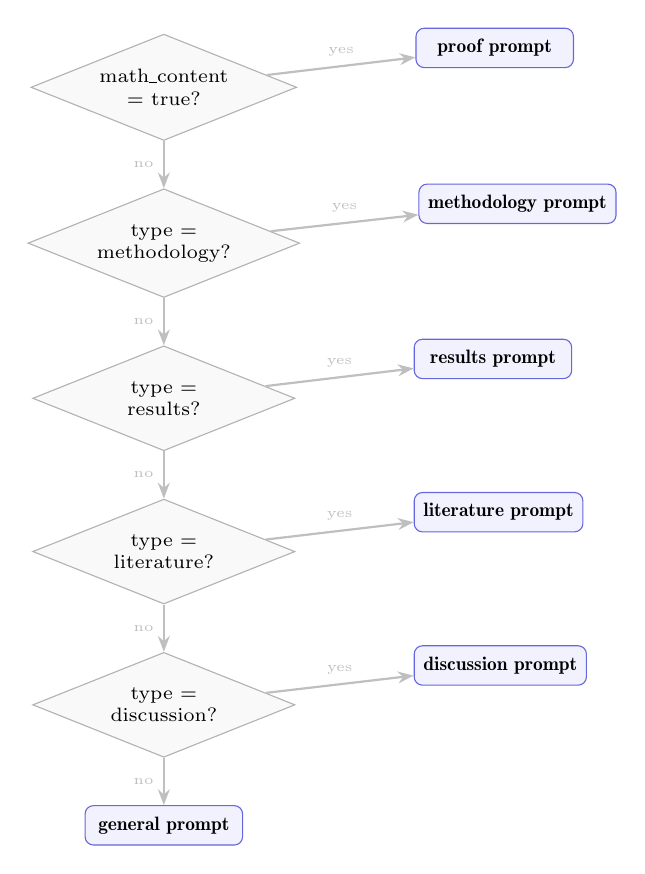
\begin{tikzpicture}[
    node distance=0.5cm,
    decision/.style={diamond, draw=gray!60, fill=gray!5, font=\scriptsize,
        aspect=2.5, inner sep=1pt, text width=2cm, align=center},
    result/.style={rectangle, rounded corners=3pt, draw=RedTitle!60, fill=blue!5,
        font=\scriptsize\bfseries, minimum width=2cm, minimum height=0.5cm, text=DarkText},
    arr/.style={-{Stealth[length=2mm]}, thick, gray!50},
]
\node[decision] (d1) {math\_content\\= true?};
\node[result, right=1.5cm of d1, yshift=0.5cm] (r1) {proof prompt};
\node[decision, below=0.6cm of d1] (d2) {type =\\methodology?};
\node[result, right=1.5cm of d2, yshift=0.5cm] (r2) {methodology prompt};
\node[decision, below=0.6cm of d2] (d3) {type =\\results?};
\node[result, right=1.5cm of d3, yshift=0.5cm] (r3) {results prompt};
\node[decision, below=0.6cm of d3] (d4) {type =\\literature?};
\node[result, right=1.5cm of d4, yshift=0.5cm] (r4) {literature prompt};
\node[decision, below=0.6cm of d4] (d5) {type =\\discussion?};
\node[result, right=1.5cm of d5, yshift=0.5cm] (r5) {discussion prompt};
\node[result, below=0.6cm of d5] (r6) {general prompt};

\draw[arr] (d1) -- node[above, font=\tiny] {yes} (r1);
\draw[arr] (d1) -- node[left, font=\tiny] {no} (d2);
\draw[arr] (d2) -- node[above, font=\tiny] {yes} (r2);
\draw[arr] (d2) -- node[left, font=\tiny] {no} (d3);
\draw[arr] (d3) -- node[above, font=\tiny] {yes} (r3);
\draw[arr] (d3) -- node[left, font=\tiny] {no} (d4);
\draw[arr] (d4) -- node[above, font=\tiny] {yes} (r4);
\draw[arr] (d4) -- node[left, font=\tiny] {no} (d5);
\draw[arr] (d5) -- node[above, font=\tiny] {yes} (r5);
\draw[arr] (d5) -- node[left, font=\tiny] {no} (r6);
\end{tikzpicture}
\end{center}

\vspace{0.1cm}
Each prompt variant focuses attention on what matters for that section type. The \textbf{proof prompt} re-derives each step; the \textbf{methodology prompt} checks identification assumptions; the \textbf{results prompt} verifies numerical consistency.

\end{frame}

%-----------------------------------------------------------
\begin{frame}{The Proof Verification Chain}

For sections with mathematical content, the skill uses a \textbf{two-pass adversarial architecture}:

\vspace{0.3cm}
\begin{center}
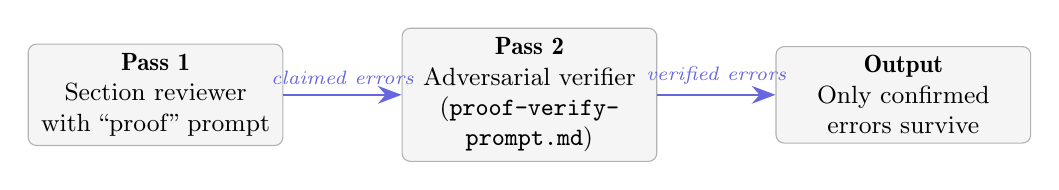
\begin{tikzpicture}[
    box/.style={rectangle, rounded corners=3pt, draw=gray!60, fill=gray!8,
        minimum width=3.2cm, minimum height=1.0cm, font=\small, text=DarkText,
        text width=3.0cm, align=center},
    arr/.style={-{Stealth[length=3mm]}, thick, RedTitle!60},
]
\node[box] (pass1) {\textbf{Pass 1}\\Section reviewer\\with ``proof'' prompt};
\node[box, right=1.5cm of pass1] (pass2) {\textbf{Pass 2}\\Adversarial verifier\\(\texttt{proof-verify-prompt.md})};
\node[box, right=1.5cm of pass2] (output) {\textbf{Output}\\Only confirmed\\errors survive};

\draw[arr] (pass1) -- node[above, font=\scriptsize\itshape] {claimed errors} (pass2);
\draw[arr] (pass2) -- node[above, font=\scriptsize\itshape] {verified errors} (output);
\end{tikzpicture}
\end{center}

\vspace{0.3cm}
\begin{itemize}
    \item \textbf{Pass 1}: Section reviewer finds potential proof issues
    \item \textbf{Pass 2}: Independent verifier re-derives each claimed error from scratch
    \item Only errors confirmed by \emph{both} passes survive
    \item If the verifier cannot reproduce the error $\Rightarrow$ the comment is dropped
\end{itemize}

\vspace{0.2cm}
\textbf{Analogy:} Two referees independently check the math. A claimed error must be confirmed by both before it reaches the author.

\end{frame}

%-----------------------------------------------------------
\begin{frame}{The MPE Paper Through the Pipeline: Phase 1}

\textbf{Phase 1: Extract \& Structure}

\vspace{0.2cm}
The pipeline reads \texttt{MPE\_Hyper\_v44.tex} and produces:

\vspace{0.2cm}
\begin{small}
\begin{tabular}{lll}
\toprule
\textbf{Section} & \textbf{Type} & \textbf{math\_content} \\
\midrule
1. Introduction & introduction & false \\
2. The Neoclassical Growth Model & methodology & true \\
3. Existence of Markov Equilibria & proof & true \\
4. The $(\beta,\delta)$-Tradeoff & results & true \\
5. Steady State Stability & proof & true \\
6. Numerical Simulations & results & false \\
7. Concluding Remarks & discussion & false \\
A. Appendix (Proofs) & proof & true \\
\bottomrule
\end{tabular}
\end{small}

\vspace{0.3cm}
\textbf{Key claims extracted:}
\begin{itemize}
    \item Theorem 1: Existence of Markov equilibrium via $\varepsilon$-equilibria
    \item Theorem 2: Saddle-path stability of steady states
    \item Proposition 1: Differentiability properties of the equilibrium map
\end{itemize}

The pipeline sees the same structure you see --- but classifies sections to route them.

\end{frame}

%-----------------------------------------------------------
\begin{frame}{The MPE Paper Through the Pipeline: Phases 2--3}

\textbf{Phase 2: Calibrate (3 parallel agents)}

\vspace{0.1cm}
\begin{small}
\begin{tabular}{lp{9cm}}
\toprule
\textbf{Agent} & \textbf{Output} \\
\midrule
Domain calibration & ``Dynamic macro theory, quasi-hyperbolic preferences, Markov equilibrium. Review criteria: check equilibrium definition, verify convergence arguments, assess numerical accuracy.'' \\
Literature search & Harris-Laibson (2001), Krusell-Kuruscu-Smith (2002), Cao-Werning (2018), \ldots \\
Contribution extraction & (1) Existence via $\varepsilon$-equilibria, (2) Saddle-path stability, (3) Numerical algorithm \\
\bottomrule
\end{tabular}
\end{small}

\vspace{0.3cm}
\textbf{Phase 3: Overview}

Generates 4--8 macro-level issues, e.g.:
\begin{itemize}
    \item \textbf{Assumption scope}: Are the concavity conditions in Assumption 2 stronger than needed for the stability result?
    \item \textbf{Numerical validation}: The paper reports accuracy for a single parameterization --- how sensitive are the results to $\beta$?
    \item \textbf{Literature positioning}: How does the $\varepsilon$-equilibrium approach compare to the viscosity solution method in Cao-Werning (2018)?
\end{itemize}

\end{frame}

%-----------------------------------------------------------
\begin{frame}{The MPE Paper Through the Pipeline: Phase 4}

\textbf{Phase 4: Section-level reviews with specialized prompts}

\vspace{0.3cm}
\begin{small}
\begin{tabular}{lp{4cm}p{6cm}}
\toprule
\textbf{Section} & \textbf{Prompt Variant} & \textbf{Focus} \\
\midrule
\S 2 (Growth Model) & methodology & Check model assumptions, identification of equilibrium, completeness of setup \\
\S 3 (Existence) & proof + verify chain & Step-by-step verification of Theorem 1; check measurability, convergence \\
\S 4 ($\beta,\delta$-Tradeoff) & results & Numerical consistency, internal coherence of comparative statics \\
\S 5 (Stability) & proof + verify chain & Verify saddle-path stability argument, check eigenvalue claims \\
\S 6 (Simulations) & results & Code reproducibility, accuracy metrics, sensitivity \\
\S 7 (Conclusion) & discussion & Do claims match formal results? \\
Appendix & proof + verify chain & Verify supporting lemmas \\
\bottomrule
\end{tabular}
\end{small}

\vspace{0.3cm}
Each section gets its own agent with the appropriate prompt variant. Sections 3, 5, and the Appendix also get the two-pass proof verification chain.

\end{frame}

%-----------------------------------------------------------
\begin{frame}{The Editorial Filter: 7 Steps}

Phase 6 applies a 7-step quality gate to all accumulated comments:

\vspace{0.2cm}
\begin{enumerate}
    \item \textbf{Remove low-value comments}: generic advice (``the authors should discuss limitations''), formatting notes, OCR artifacts, restated overview issues

    \vspace{0.1cm}
    \item \textbf{Contradiction check}: Does any comment contradict the paper's own stated defense? (Check footnotes, remarks)

    \vspace{0.1cm}
    \item \textbf{Quote verification}: Exact character-for-character match against the full paper text. Fuzzy match $>80\%$ $\Rightarrow$ accept. No match $\Rightarrow$ \textbf{drop the comment}

    \vspace{0.1cm}
    \item \textbf{Severity assignment}: critical / major / minor; confidence: high / medium / low

    \vspace{0.1cm}
    \item \textbf{Notation capping}: Max 2--3 purely notational comments (diminishing returns)

    \vspace{0.1cm}
    \item \textbf{Humanize language}: Vary sentence openers, remove banned AI vocabulary, ensure natural cadence

    \vspace{0.1cm}
    \item \textbf{Order by importance}: critical $\to$ major $\to$ minor; high confidence first within each tier
\end{enumerate}

\vspace{0.2cm}
$\Rightarrow$ Without this filter, you get 40 comments. After it, you get 12--20 --- each substantive, correctly quoted, and ordered by severity.

\end{frame}

%-----------------------------------------------------------
\begin{frame}{Quote Verification: The Final Defense}

The most embarrassing failure mode: a review comment that ``quotes'' something the paper never said.

\vspace{0.3cm}
\textbf{The verification rule:}
\begin{center}
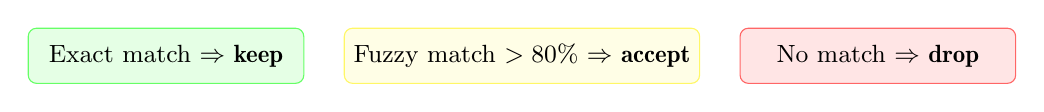
\begin{tikzpicture}[
    box/.style={rectangle, rounded corners=3pt, draw=gray!60, fill=gray!8,
        minimum height=0.7cm, font=\small, text=DarkText, minimum width=3.5cm},
    arr/.style={-{Stealth[length=2.5mm]}, thick, gray!50},
]
\node[box, fill=green!10, draw=green!60] (exact) {Exact match $\Rightarrow$ \textbf{keep}};
\node[box, fill=yellow!10, draw=yellow!60, right=0.5cm of exact] (fuzzy) {Fuzzy match $>80\%$ $\Rightarrow$ \textbf{accept}};
\node[box, fill=red!10, draw=red!60, right=0.5cm of fuzzy] (none) {No match $\Rightarrow$ \textbf{drop}};
\end{tikzpicture}
\end{center}

\vspace{0.3cm}
\textbf{Quote requirements} (from \texttt{shared-directives.md}):
\begin{itemize}
    \item Exact character-for-character copy, including \LaTeX{} commands (\texttt{\textbackslash rho}, \texttt{\textbackslash frac})
    \item Complete passages --- never truncate mid-sentence
    \item Multi-line equations: include ALL lines
    \item Minimum 2 full sentences or complete equation block
\end{itemize}

\vspace{0.3cm}
\textbf{Safety fallback:} If quote verification would drop ALL comments (e.g., because the PDF extraction mangled the text), skip verification and keep originals. This prevents silent failure.

\end{frame}


%===========================================================
% SECTION: CASE STUDY 1 --- RUNNING AND OUTPUT
%===========================================================
\section{Case Study 1: Running and Output}

%-----------------------------------------------------------
\begin{frame}[fragile]{Installation: Two Lines}

\begin{lstlisting}[style=bashstyle]
# Copy the skill folder into your project
cp -r review-paper-skill/ .claude/commands/review-paper/
\end{lstlisting}

\vspace{0.3cm}
That's it. A skill is a folder. Installation is copying a folder.

\vspace{0.3cm}
\textbf{What this does:}
\begin{itemize}
    \item Claude Code discovers any \texttt{SKILL.md} files in \texttt{.claude/commands/}
    \item The YAML frontmatter registers the skill name and trigger phrases
    \item From now on, typing \texttt{/review-paper} or saying ``review this paper'' activates the skill
\end{itemize}

\vspace{0.3cm}
\textbf{No compilation. No API keys. No dependencies.}\\
The skill runs entirely within Claude Code's existing infrastructure.

\end{frame}

%-----------------------------------------------------------
\begin{frame}[fragile]{Invocation: One Command}

\begin{lstlisting}[style=bashstyle]
/review-paper MPE_Hyper_v44.pdf
\end{lstlisting}

\vspace{0.3cm}
\textbf{Optional flags:}
\begin{small}
\begin{tabular}{lp{9cm}}
\toprule
\textbf{Flag} & \textbf{Effect} \\
\midrule
\texttt{--cheap} & Shorter review: fewer section agents, skip literature search \\
\texttt{--no-literature} & Skip the WebSearch for related papers \\
\texttt{--output path/to/out.md} & Custom output path (default: \texttt{MPE\_Hyper\_v44\_review.md}) \\
\bottomrule
\end{tabular}
\end{small}

\vspace{0.3cm}
\textbf{Input formats supported:} PDF, TeX, TXT, Markdown, DOCX, HTML, EPUB.

\vspace{0.2cm}
For the demo, we use the \texttt{.tex} source directly --- Claude reads \LaTeX{} natively, preserving all mathematical notation.

\end{frame}

%-----------------------------------------------------------
\begin{frame}{What Happens Under the Hood}

\textbf{Timeline of a typical run} (on a 40-page macro theory paper):

\vspace{0.3cm}
\begin{center}
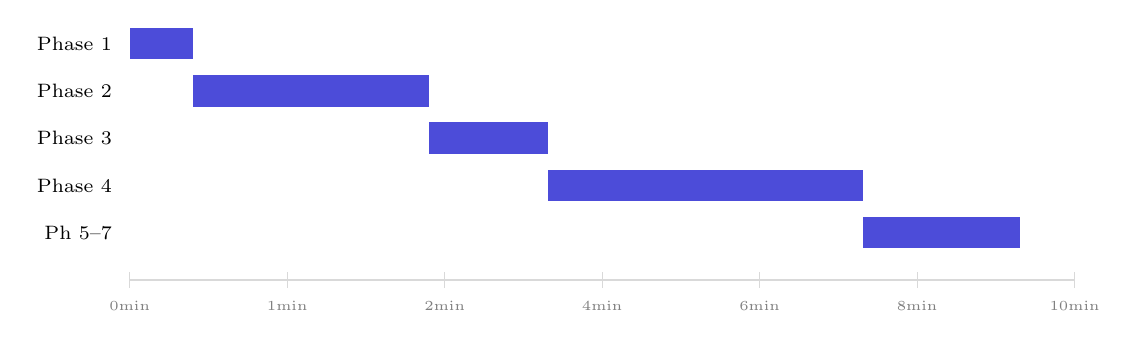
\begin{tikzpicture}[
    bar/.style={rectangle, minimum height=0.4cm, font=\scriptsize, text=white, anchor=west},
    label/.style={font=\scriptsize, anchor=east, text=DarkText},
]
\draw[thick, gray!30] (0,0) -- (12,0);
\foreach \x/\t in {0/0, 2/1, 4/2, 6/4, 8/6, 10/8, 12/10} {
    \draw[gray!30] (\x,-0.1) -- (\x,0.1);
    \node[below, font=\tiny, text=gray] at (\x,-0.15) {\t min};
}

\node[label] at (-0.1, 3.0) {Phase 1};
\node[bar, fill=RedTitle!70, minimum width=0.8cm] at (0, 3.0) {};

\node[label] at (-0.1, 2.4) {Phase 2};
\node[bar, fill=RedTitle!70, minimum width=3.0cm] at (0.8, 2.4) {};

\node[label] at (-0.1, 1.8) {Phase 3};
\node[bar, fill=RedTitle!70, minimum width=1.5cm] at (3.8, 1.8) {};

\node[label] at (-0.1, 1.2) {Phase 4};
\node[bar, fill=RedTitle!70, minimum width=4.0cm] at (5.3, 1.2) {};

\node[label] at (-0.1, 0.6) {Ph 5--7};
\node[bar, fill=RedTitle!70, minimum width=2.0cm] at (9.3, 0.6) {};
\end{tikzpicture}
\end{center}

\vspace{0.2cm}
\begin{small}
\begin{tabular}{lll}
\toprule
\textbf{Phase} & \textbf{Duration} & \textbf{Why} \\
\midrule
1: Extract & $\sim$30s & Read paper, parse sections \\
2: Calibrate & $\sim$2 min & 3 parallel agents (literature search is the bottleneck) \\
3: Overview & $\sim$1 min & Single agent, uses calibration output \\
4: Section Reviews & $\sim$3--5 min & $N$ parallel agents + proof verification chain \\
5--7: Filter + Render & $\sim$2 min & Cross-section, editorial filter, output synthesis \\
\midrule
\textbf{Total} & \textbf{$\sim$8--10 min} & \\
\bottomrule
\end{tabular}
\end{small}

\end{frame}

%-----------------------------------------------------------
\begin{frame}[fragile]{The Output: refine.ink Format}

\begin{lstlisting}[style=markdownstyle, basicstyle=\ttfamily\scriptsize]
# Markov Equilibria with Quasi-Hyperbolic Discounting

**Date**: 04/11/2026
**Domain**: social_sciences/economics
**Taxonomy**: academic/research_paper
**Filter**: Active comments

---
## Overall Feedback

**Assumption scope may be stronger than needed**
Assumption 2 imposes strict concavity on the composite
return function. However, the stability argument in
Section 5 only requires local concavity near the steady
state. Relaxing this would broaden applicability to
models with non-smooth production technologies...

**Recommendation**: Minor revision
**Key revision targets**:
1. Clarify necessity of global vs. local concavity
2. Add sensitivity analysis across beta values
\end{lstlisting}

\vspace{0.1cm}
Each overview issue: 4--8 sentences with specific section and equation references.

\end{frame}

%-----------------------------------------------------------
\begin{frame}[fragile]{The Output: Detailed Comments}

\begin{lstlisting}[style=markdownstyle, basicstyle=\ttfamily\scriptsize]
## Detailed Comments (14)

### 1. Measurability gap in epsilon-equilibrium construction
**Status**: Pending
**Quote**:
> "For each $\varepsilon > 0$, let $W_\varepsilon$ denote
> the policy function solving the truncated problem (3.2).
> The sequence $\{W_\varepsilon\}$ converges pointwise..."

**Feedback**:
The convergence claim needs the sequence to be measurable
with respect to the product sigma-algebra. The paper
establishes pointwise convergence but does not verify
that the limit function inherits measurability from the
approximants. Since the state space includes both capital
and the exogenous shock, this is not automatic. Consider
adding a brief measurability argument via Lemma A.2.
\end{lstlisting}

\vspace{0.1cm}
Each comment: verbatim quote $\to$ substantive feedback $\to$ concrete remediation.

\end{frame}

%-----------------------------------------------------------
\begin{frame}{What You Do With the Output}

The skill output is a \textbf{draft}, not a finished review.

\vspace{0.3cm}
\textbf{The economist's role (Pillar 5 --- Verify):}

\vspace{0.2cm}
\begin{columns}[T]
\begin{column}{0.48\textwidth}
\textbf{You must check:}
\begin{enumerate}
    \item Math claims --- re-derive any flagged errors
    \item Domain judgment --- does the critique match field standards?
    \item Missing context --- papers the agent couldn't access
    \item Tone --- appropriate for the venue?
\end{enumerate}
\end{column}

\begin{column}{0.48\textwidth}
\textbf{The skill handles:}
\begin{enumerate}
    \item Systematic extraction of claims
    \item Cross-referencing sections
    \item Quote grounding
    \item Ordering by severity
    \item Format consistency
\end{enumerate}
\end{column}
\end{columns}

\vspace{0.4cm}
\textbf{Think of it as:} The skill writes the first draft of a referee report in 10 minutes. You spend 30 minutes verifying and editing. Total: 40 minutes instead of 4 hours.

\vspace{0.2cm}
\textbf{The skill does not replace your judgment.} It replaces the mechanical parts of refereeing: extraction, cross-referencing, quote verification, formatting.

\end{frame}


%===========================================================
% SECTION: CASE STUDY 2 --- THE PROBLEM
%===========================================================
\section{Case Study 2: The Problem}

%-----------------------------------------------------------
\begin{frame}{The Naive Baseline: 24 Files, 24 Headaches}

\textbf{Scenario:} You want the US uninsurance rate, 2000--2023, broken down by demographics.

\vspace{0.2cm}
\textbf{The naive approach:}
\begin{enumerate}
    \item Go to the MEPS website (\texttt{meps.ahrq.gov})
    \item Download 24 Full Year Consolidated files (one per year)
    \item Open each in Stata/R, figure out the variable names
    \item Merge all 24 years
    \item Compute weighted statistics
    \item Make plots
\end{enumerate}

\vspace{0.2cm}
\textbf{Four failure modes you will encounter:}
\begin{enumerate}
    \item \textbf{Variable names change:} \texttt{INSCOV01} in 2001 vs.\ \texttt{INSCOV22} in 2022
    \item \textbf{File formats shift:} SAS transport (.ssp) with varying internal structure
    \item \textbf{Weight variables change names:} \texttt{PERWT01F} vs.\ \texttt{PERWT22F}
    \item \textbf{Silent merge errors:} You make a crosswalk mistake on year 14 and don't notice until a referee asks why your 2014 number is wrong
\end{enumerate}

\end{frame}

%-----------------------------------------------------------
\begin{frame}{The Research Question}

\begin{tcolorbox}[colback=blue!3, colframe=RedTitle!60]
\textbf{Who is uninsured in the United States, 2000--2023?}\\
How has the uninsurance rate evolved, and how did the Affordable Care Act change the distribution?
\end{tcolorbox}

\vspace{0.3cm}
\textbf{Why this matters for macroeconomics:}
\begin{itemize}
    \item Health insurance is a major \textbf{incomplete market} --- uninsured households face uninsurable medical expenditure risk
    \item The ACA (2010/2014) was the largest expansion of social insurance since Medicare (1965)
    \item Understanding \emph{who} gained coverage informs \textbf{welfare analysis} of the policy
    \item Heterogeneous-agent macro models (Lec06) require calibrated distributions of insurance status
\end{itemize}

\vspace{0.3cm}
\textbf{Sub-questions:}
\begin{itemize}
    \item How does uninsurance vary by age, income, race, employment, and region?
    \item Which groups saw the largest coverage gains from the ACA?
    \item Are there persistent disparities even after the ACA?
\end{itemize}

\end{frame}

%-----------------------------------------------------------
\begin{frame}{What PaulGP Did with HMDA (The Parallel)}

\textbf{Reference:} Paul Goldsmith-Pinkham, ``Large Datasets and Structured Databases,'' 2026.

\vspace{0.2cm}
\begin{small}
\begin{tabular}{lp{9cm}}
\toprule
\textbf{Stage} & \textbf{What He Did} \\
\midrule
Data & HMDA mortgage data: 291M applications, 2007--2024, $\sim$70 GB of CSVs \\
Download & Claude Code fetched files from CFPB with resume capability \\
Convert & CSV $\to$ Parquet (15$\times$ compression) \\
Harmonize & Pre-2018 vs.\ post-2018 schema differences, lender ID crosswalks \\
Analyze & County-by-year tables: origination counts, denial rates, HHI \\
Visualize & Fintech origination share (1.1\% in 2007 $\to$ 16.3\% peak in 2021) \\
\bottomrule
\end{tabular}
\end{small}

\vspace{0.3cm}
\textbf{Key insight from the article:}
\begin{quote}
{\footnotesize\itshape ``The fixed cost of doing this properly has collapsed. What used to require a data engineer and weeks of pipeline work, Claude Code does in a single session.''}
\end{quote}

\vspace{0.2cm}
\textbf{We do the same thing with MEPS data.}

\end{frame}

%-----------------------------------------------------------
\begin{frame}{Our Workflow: HMDA $\leftrightarrow$ MEPS Mapping}

\begin{small}
\begin{tabular}{p{4.5cm}p{5cm}p{3.5cm}}
\toprule
\textbf{PaulGP (HMDA)} & \textbf{Our Workflow (MEPS)} & \textbf{Challenge} \\
\midrule
Download CSVs from CFPB & Download .ssp files from AHRQ & Different host, format \\
Convert CSV $\to$ Parquet & Convert .ssp $\to$ pandas DataFrames & Need \texttt{pyreadstat} \\
Harmonize pre/post-2018 schemas & Harmonize variable names across years & \texttt{INSCOV01} $\to$ \texttt{INSCOV22} \\
Build DuckDB database & Build merged panel DataFrame & Simpler for our scale \\
Run aggregation queries & Compute weighted statistics by group & MEPS weights are critical \\
Generate HMDA figures & Generate 6 MEPS figures & Different story, same arc \\
\bottomrule
\end{tabular}
\end{small}

\vspace{0.4cm}
\textbf{Three-phase architecture:}
\begin{enumerate}
    \item \textbf{Phase A:} Data acquisition \& cleaning (download, convert, harmonize)
    \item \textbf{Phase B:} Analysis pipeline (weighted aggregation by year $\times$ group)
    \item \textbf{Phase C:} Visualization (6 figures with ACA/COVID annotations)
\end{enumerate}

\vspace{0.2cm}
\textbf{No skill needed.} This is a single Claude Code session with 3 prompts.

\end{frame}


%===========================================================
% SECTION: CASE STUDY 2 --- DATA ARCHITECTURE
%===========================================================
\section{Case Study 2: Data Architecture}

%-----------------------------------------------------------
\begin{frame}[fragile]{The Claude Code Prompt for Phase A}

\begin{lstlisting}[style=pythonstyle, language={}, basicstyle=\ttfamily\scriptsize]
I want to analyze uninsurance rates in the US from
2000 to 2023 using MEPS data from AHRQ.

Download the Full Year Consolidated files for each year.
The files are in SAS transport format (.ssp).

Parse each file. Extract these variables:
- Insurance coverage (INSCOV / INSCOVY)
- Age (AGELAST)
- Race/ethnicity (RACETHX)
- Poverty category (POVCAT)
- Census region (REGION)
- Employment status (EMPST)
- Sex (SEX)
- Person-level weight (PERWT / PERWTF)

Harmonize variable names across years (they are
year-suffixed, e.g. INSCOV01, INSCOV22).

Save as a single parquet file: meps_panel_2000_2023.parquet
\end{lstlisting}

\vspace{0.1cm}
\textbf{One prompt.} Claude figures out the AHRQ URLs, downloads 24 files, parses each, harmonizes the variable names, and saves the result.

\end{frame}

%-----------------------------------------------------------
\begin{frame}[fragile]{What Claude Does Autonomously}

\textbf{Given the prompt, Claude Code:}

\vspace{0.2cm}
\begin{enumerate}
    \item \textbf{Discovers the URL pattern}: MEPS files follow \texttt{https://meps.ahrq.gov/data\_files/pufs/hNNNssp.zip} where \texttt{NNN} is the file number (HC-028 for 2000, HC-233 for 2023)

    \vspace{0.1cm}
    \item \textbf{Handles obstacles}: Some years return 403 errors $\to$ adds \texttt{User-Agent} header. Some files have different encoding $\to$ tries multiple parsers.

    \vspace{0.1cm}
    \item \textbf{Builds a crosswalk dictionary}:
    \begin{small}
    \begin{verbatim}
    crosswalk = {
      2001: {'INSCOV01': 'INSCOV', 'PERWT01F': 'PERWT', ...},
      2022: {'INSCOV22': 'INSCOV', 'PERWT22F': 'PERWT', ...},
    }
    \end{verbatim}
    \end{small}

    \vspace{0.1cm}
    \item \textbf{Validates}: Checks that insurance coverage variable has values \{1, 2, 3\} (Private, Public, Uninsured) in every year. Flags anomalies.

    \vspace{0.1cm}
    \item \textbf{Merges and saves}: Stacks all years into a single DataFrame, writes Parquet.
\end{enumerate}

\vspace{0.2cm}
\textbf{Time:} $\sim$5--10 minutes for all 24 years.

\end{frame}

%-----------------------------------------------------------
\begin{frame}{Schema Harmonization: The Hard Part}

\textbf{The core challenge:} MEPS variable names are \emph{year-suffixed}.

\vspace{0.3cm}
\begin{small}
\begin{tabular}{lccc}
\toprule
\textbf{Concept} & \textbf{Year 2001} & \textbf{Year 2014} & \textbf{Year 2022} \\
\midrule
Insurance coverage & \texttt{INSCOV01} & \texttt{INSCOV14} & \texttt{INSCOV22} \\
Person weight & \texttt{PERWT01F} & \texttt{PERWT14F} & \texttt{PERWT22F} \\
Age at end of year & \texttt{APTS42} or \texttt{APTS53} & \texttt{AGELAST} & \texttt{AGELAST} \\
Employment status & \texttt{EMPST31} & \texttt{EMPST31} & \texttt{EMPST31} \\
\bottomrule
\end{tabular}
\end{small}

\vspace{0.3cm}
\textbf{Additional complications:}
\begin{itemize}
    \item Pre-2014 vs.\ post-2014: The ACA changed what ``public coverage'' means
    \item Race/ethnicity categories expanded over time
    \item Some variables were renamed without changing content
\end{itemize}

\vspace{0.3cm}
\textbf{Why this is perfect for an agent:}
\begin{itemize}
    \item Tedious for humans (24 years $\times$ 8 variables = 192 name lookups)
    \item Error-prone for humans (one wrong mapping $\Rightarrow$ silent bias)
    \item Well-suited for an agent that can read MEPS documentation
\end{itemize}

\end{frame}

%-----------------------------------------------------------
\begin{frame}{The Merged Dataset}

After harmonization:

\vspace{0.3cm}
\begin{small}
\begin{tabular}{lp{10cm}}
\toprule
\textbf{Property} & \textbf{Value} \\
\midrule
Rows & $\sim$500K--800K (varies by year; $\sim$25K--35K respondents per year $\times$ 24 years) \\
Columns & \texttt{YEAR}, \texttt{INSCOV} (1/2/3), \texttt{AGELAST}, \texttt{RACETHX}, \texttt{POVCAT}, \texttt{REGION}, \texttt{EMPST}, \texttt{SEX}, \texttt{PERWT} \\
Key variable & \texttt{INSCOV}: 1=Any Private, 2=Public Only, 3=Uninsured \\
Weight & \texttt{PERWT}: person-level survey weight for nationally representative estimates \\
\bottomrule
\end{tabular}
\end{small}

\vspace{0.3cm}
\textbf{From 24 separate files with inconsistent naming to one clean panel.}

\vspace{0.2cm}
This is the data architecture step in the PaulGP framework: the boring but critical infrastructure that makes all downstream analysis possible.

\vspace{0.2cm}
\textbf{The agent did in 10 minutes what would take a careful RA half a day.}

\end{frame}

%-----------------------------------------------------------
\begin{frame}[fragile]{The Prompt for Phase B: Analysis}

\begin{lstlisting}[style=pythonstyle, language={}, basicstyle=\ttfamily\scriptsize]
Using the merged MEPS data, compute the weighted
uninsurance rate (INSCOV == 3) by year, overall
and broken down by:
  - age group (18-25, 26-34, 35-44, 45-54, 55-64)
  - poverty category (Poor, Near Poor, Low Income,
    Middle Income, High Income)
  - race/ethnicity (White NH, Black NH, Hispanic, Asian)
  - employment status
  - Census region

Use person weights (PERWT) for nationally representative
estimates. Uninsurance rate = sum(PERWT where INSCOV==3)
                            / sum(PERWT)

Save the aggregated statistics as CSV files.
\end{lstlisting}

\vspace{0.1cm}
\textbf{Second prompt.} Claude computes all group-level statistics with proper weighting.

\end{frame}

%-----------------------------------------------------------
\begin{frame}{Weighted Statistics: Why Weighting Matters}

\textbf{MEPS uses a complex survey design.} Each respondent represents a different number of people in the US population.

\vspace{0.3cm}
\textbf{For each year $\times$ group:}
\[
\text{Uninsurance rate} = \frac{\sum_{i \in \text{group}} w_i \cdot \mathbf{1}[\text{INSCOV}_i = 3]}{\sum_{i \in \text{group}} w_i}
\]
where $w_i$ = \texttt{PERWT} (person-level weight).

\vspace{0.3cm}
\textbf{Why unweighted estimates are wrong:}
\begin{itemize}
    \item MEPS oversamples certain populations (low-income, minority groups) for precision
    \item Unweighted statistics overcount these groups relative to their population share
    \item Example: unweighted uninsurance rate might be 18\%; weighted rate is 13\%
\end{itemize}

\vspace{0.3cm}
\textbf{Claude knows this} --- if you mention ``person weights'' in the prompt, it applies them correctly. But you must \emph{check}: this is Pillar 5 in action.

\end{frame}

%-----------------------------------------------------------
\begin{frame}{Validation: Trust But Verify}

\textbf{Cross-check against known statistics:}

\vspace{0.2cm}
\begin{small}
\begin{tabular}{lcc}
\toprule
\textbf{Year} & \textbf{Census Bureau (CPS ASEC)} & \textbf{Our MEPS Estimate} \\
\midrule
2010 & 16.3\% & Should be $\approx$15--17\% \\
2013 & 13.4\% (pre-ACA peak) & Should be $\approx$12--14\% \\
2016 & 8.8\% & Should be $\approx$8--10\% \\
2019 & 8.0\% & Should be $\approx$7--9\% \\
2022 & 7.9\% & Should be $\approx$7--9\% \\
\bottomrule
\end{tabular}
\end{small}

\vspace{0.3cm}
\textbf{Note:} MEPS and CPS use different survey designs, so exact match is not expected. But they should tell the same story:
\begin{itemize}
    \item Rising or flat before ACA ($\sim$2000--2013)
    \item Sharp drop after 2014
    \item Relatively stable 2016--2023
\end{itemize}

\vspace{0.2cm}
\textbf{If your 2013 rate is 5\% or 25\%, something is wrong.} You must know the data well enough to spot when the agent makes a mistake. This is the economist's contribution.

\end{frame}


%===========================================================
% SECTION: CASE STUDY 2 --- VISUALIZATION AND INSIGHTS
%===========================================================
\section{Case Study 2: Visualization and Insights}

%-----------------------------------------------------------
\begin{frame}[fragile]{The Prompt for Phase C: Visualization}

\begin{lstlisting}[style=pythonstyle, language={}, basicstyle=\ttfamily\scriptsize]
Generate 6 publication-quality figures showing
uninsurance rate trends 2000-2023.

Use matplotlib with a clean academic style.
Add vertical dashed lines for:
  - ACA passage (2010)
  - ACA coverage expansion (2014)
  - COVID-19 (2020)

Each figure: clear axis labels, legend, title.
Save as both PNG (300 DPI) and PDF.

Figures:
1. Overall uninsurance rate (time series)
2. By age group (18-25, 26-34, 35-44, 45-54, 55-64)
3. By poverty category
4. By race/ethnicity
5. By employment status
6. Regional heatmap (year x Census region)
\end{lstlisting}

\vspace{0.1cm}
\textbf{Third prompt.} Claude generates all 6 figures from the aggregated statistics.

\end{frame}

%-----------------------------------------------------------
\begin{frame}{Figure 1: Overall Uninsurance Rate, 2000--2023}

\begin{center}

\includegraphics[width=0.85\textwidth]{fig_overall_uninsurance.pdf}
\end{center}

\vspace{0.1cm}
\textbf{The headline story:} Uninsurance was $\sim$14--16\% through the 2000s, peaked around the Great Recession, dropped sharply after ACA coverage expansion in 2014, and stabilized around 8\% in the late 2010s.

\end{frame}

%-----------------------------------------------------------
\begin{frame}{Figure 2: By Age Group}

\begin{center}

\includegraphics[width=0.85\textwidth]{fig_uninsurance_by_age.pdf}
\end{center}

\vspace{0.1cm}
\textbf{Key insight:} The 18--25 group had the highest uninsurance rate ($\sim$28--30\% pre-ACA). The 2010 ACA dependent-coverage provision (stay on parents' insurance until age 26) produced a visible drop for this group starting in 2011 --- a \textbf{policy evaluation in one figure}.

\end{frame}

%-----------------------------------------------------------
\begin{frame}{Figure 3: By Poverty Category}

\begin{center}

\includegraphics[width=0.85\textwidth]{fig_uninsurance_by_poverty.pdf}
\end{center}

\vspace{0.1cm}
\textbf{Key insight:} The poor ($<$100\% FPL) and near-poor (100--125\% FPL) saw the largest coverage gains from Medicaid expansion. High-income groups ($>$400\% FPL) were largely unaffected --- they already had employer-sponsored insurance. The ACA was a \textbf{targeted intervention}.

\end{frame}

%-----------------------------------------------------------
\begin{frame}{Figure 4: By Race/Ethnicity}

\begin{center}

\includegraphics[width=0.85\textwidth]{fig_uninsurance_by_race.pdf}
\end{center}

\vspace{0.1cm}
\textbf{Key insight:} Hispanic Americans had the highest uninsurance rate throughout the period ($\sim$32\% pre-ACA). All groups saw coverage gains after 2014, but persistent disparities remain. These disparities are a key input for heterogeneous-agent models of health insurance markets.

\end{frame}

%-----------------------------------------------------------
\begin{frame}{Figure 5: By Employment Status}

\begin{center}

\includegraphics[width=0.85\textwidth]{fig_uninsurance_by_employment.pdf}
\end{center}

\vspace{0.1cm}
\textbf{Key insight:} The US employer-based insurance system creates a stark divide. Full-time workers have $\sim$10\% uninsurance; unemployed and part-time workers face rates 2--3$\times$ higher. The ACA compressed this gap but did not eliminate it.

\end{frame}

%-----------------------------------------------------------
\begin{frame}{Figure 6: Regional Heatmap}

\begin{center}

\includegraphics[width=0.85\textwidth]{fig_uninsurance_heatmap.pdf}
\end{center}

\vspace{0.1cm}
\textbf{Key insight:} The South consistently has the highest uninsurance rates. After 2014, states that expanded Medicaid (concentrated in the Northeast and West) show sharper declines. The regional divergence reflects the \textbf{state-level variation in ACA implementation}.

\end{frame}

%-----------------------------------------------------------
\begin{frame}{What Claude Did vs.\ What Stayed Human}

\begin{columns}[T]
\begin{column}{0.48\textwidth}
\textbf{Claude Code handled:}
\begin{itemize}
    \item Downloaded 24 files from AHRQ
    \item Discovered variable name patterns
    \item Built the year-specific crosswalk
    \item Parsed SAS transport files
    \item Merged into a clean panel
    \item Computed weighted statistics
    \item Generated 6 publication-quality figures
    \item Handled format obstacles (403 errors, encoding)
\end{itemize}
\end{column}

\begin{column}{0.48\textwidth}
\textbf{The economist provided:}
\begin{itemize}
    \item The research question
    \item Which demographic breakdowns to compute
    \item The weighting requirement
    \item Validation benchmarks (Census Bureau rates)
    \item Interpretation against economic theory
    \item Policy annotation choices (ACA, COVID)
    \item Quality judgment on the figures
\end{itemize}
\end{column}
\end{columns}

\vspace{0.4cm}
\textbf{The question and the interpretation are yours.}\\
Everything between them is accelerated.

\end{frame}


%===========================================================
% SECTION: LESSONS AND PATTERNS
%===========================================================
\section{Lessons and Patterns}

%-----------------------------------------------------------
\begin{frame}{Common Patterns Across Both Case Studies}

\begin{enumerate}
    \item \textbf{Decomposition.} Both workflows broke the task into phases:
    \begin{itemize}
        \item Paper review: 7 sequential phases with within-phase parallelism
        \item MEPS analysis: 3 phases (download $\to$ analyze $\to$ visualize)
    \end{itemize}

    \vspace{0.2cm}
    \item \textbf{Domain knowledge encoding.}
    \begin{itemize}
        \item Paper review: \texttt{shared-directives.md} encodes refereeing norms
        \item MEPS: the prompt specifies weighting, variable names, validation targets
    \end{itemize}

    \vspace{0.2cm}
    \item \textbf{Validation as a first-class step.}
    \begin{itemize}
        \item Paper review: quote verification, proof verification chain, editorial filter
        \item MEPS: cross-check against Census Bureau published statistics
    \end{itemize}

    \vspace{0.2cm}
    \item \textbf{The PaulGP arc:} Problem $\to$ Infrastructure $\to$ Architecture $\to$ Capability $\to$ Insights.
    \begin{itemize}
        \item Both workflows followed this arc naturally
        \item The arc works because it separates the ``what'' (your question) from the ``how'' (the agent's execution)
    \end{itemize}
\end{enumerate}

\end{frame}

%-----------------------------------------------------------
\begin{frame}{When to Build a Skill vs.\ Use Ad Hoc Prompts}

\begin{small}
\begin{tabular}{p{6cm}p{6cm}}
\toprule
\textbf{Build a Skill When\ldots} & \textbf{Use Ad Hoc Prompts When\ldots} \\
\midrule
You will repeat the workflow $>$3 times & The task is one-off \\
The workflow has $>$5 interdependent steps & The task is simple (1--3 prompts) \\
Quality control matters (editorial filter, verification) & You are exploring and don't know the workflow yet \\
You want reproducibility across users/projects & The output format is flexible \\
Multiple people will use the workflow & Only you need this analysis \\
\bottomrule
\end{tabular}
\end{small}

\vspace{0.3cm}
\textbf{Case Study 1} (paper review): A skill. You will review many papers; quality control is essential; the 7-phase pipeline is complex; other researchers can reuse it.

\vspace{0.2cm}
\textbf{Case Study 2} (MEPS analysis): Ad hoc. One-off exploration; 3 prompts; output is a set of figures that you'll refine interactively.

\vspace{0.2cm}
\textbf{Rule of thumb:} If you're about to copy-paste the same prompt for the third time, it's time to build a skill.

\end{frame}

%-----------------------------------------------------------
\begin{frame}{Prompt Engineering Principles from the Skill}

Five principles extracted from \texttt{shared-directives.md} that apply to \emph{any} prompt:

\vspace{0.3cm}
\begin{enumerate}
    \item \textbf{Ban specific failure modes by name.}\\
    Don't say ``write naturally.'' Say ``NEVER use `crucial,' `comprehensive,' `robust.'\,'' Explicit bans are more effective than vague aspirations.

    \vspace{0.15cm}
    \item \textbf{Require concrete evidence for claims.}\\
    The confidence gate: ``Only assert an error if you can derive it step-by-step.'' Prevents hallucinated findings.

    \vspace{0.15cm}
    \item \textbf{Specify the output format precisely.}\\
    \texttt{output-format.md} defines every heading, every field, every separator. Eliminates format negotiation.

    \vspace{0.15cm}
    \item \textbf{Include anti-hallucination checks.}\\
    Quote verification, the contribution inversion test. Build skepticism into the pipeline.

    \vspace{0.15cm}
    \item \textbf{Use reference examples.}\\
    The reference-example folder shows the gold standard. ``Make your output look like this'' is the most effective prompt pattern.
\end{enumerate}

\end{frame}

%-----------------------------------------------------------
\begin{frame}{The Division of Labor}

\begin{small}
\begin{tabular}{p{6cm}p{6cm}}
\toprule
\textbf{You Provide} & \textbf{AI Provides} \\
\midrule
Research question (``who is uninsured?'') & Data download and format conversion \\
Domain knowledge (which MEPS variables matter) & Schema harmonization across 24 years \\
Economic interpretation (ACA effects on welfare) & Weighted statistics computation \\
Judgment (``is this review comment valid?'') & Quote verification against source text \\
Quality standard (what a good review looks like) & Mechanical filtering and ordering \\
Validation benchmarks (Census Bureau rates) & Cross-checking computations \\
\bottomrule
\end{tabular}
\end{small}

\vspace{0.4cm}
\textbf{The pattern:} You provide the \emph{why} and the \emph{what}. The agent provides the \emph{how}.

\vspace{0.2cm}
This is not a replacement. It is a \textbf{division of labor} that lets you focus on what you are uniquely good at: asking the right question, knowing what a correct answer looks like, and interpreting the results against economic theory.

\end{frame}

%-----------------------------------------------------------
\begin{frame}{Failure Modes to Watch For}

\begin{columns}[T]
\begin{column}{0.48\textwidth}
\textbf{Paper Review Failures}
\begin{enumerate}
    \item \textbf{Hallucinated math errors:} The model says a proof step is wrong, but it isn't. Mitigation: two-pass verification chain.

    \vspace{0.1cm}
    \item \textbf{Generic comments survive:} ``The authors should discuss limitations.'' Mitigation: editorial filter step 1.

    \vspace{0.1cm}
    \item \textbf{Missing context:} Papers the agent can't access (paywalled references). Mitigation: you fill in.
\end{enumerate}
\end{column}

\begin{column}{0.48\textwidth}
\textbf{Data Analysis Failures}
\begin{enumerate}
    \item \textbf{Wrong variable crosswalk:} Silent errors --- the uninsurance rate for 2014 looks wrong. Mitigation: validate against published benchmarks.

    \vspace{0.1cm}
    \item \textbf{Unweighted statistics:} Biased estimates because survey weights were dropped. Mitigation: explicitly require weighting in the prompt.

    \vspace{0.1cm}
    \item \textbf{Missing data as zeros:} AI treats missing insurance status as ``insured.'' Mitigation: check for \texttt{NaN} handling.
\end{enumerate}
\end{column}
\end{columns}

\vspace{0.3cm}
\textbf{Both failure modes require domain expertise to detect.} This is why the 5-pillar workflow (Lec09) is non-negotiable: the verification pillar is your defense.

\end{frame}

%-----------------------------------------------------------
\begin{frame}{Looking Back at the Course}

\begin{center}
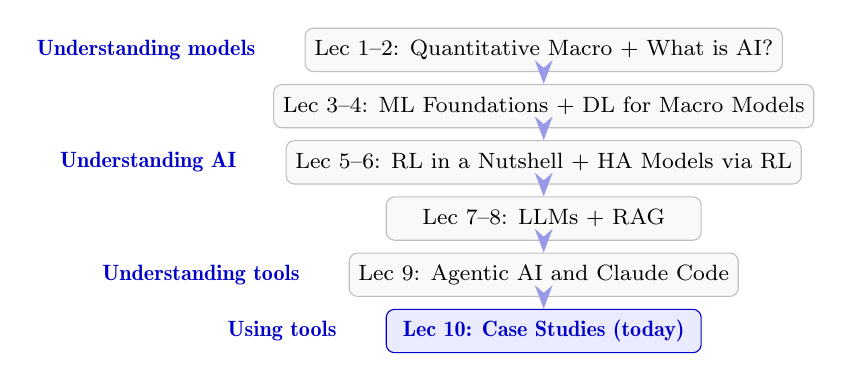
\begin{tikzpicture}[
    node distance=0.15cm,
    block/.style={rectangle, rounded corners=3pt, draw=gray!50, fill=gray!5,
        minimum width=4cm, minimum height=0.55cm, font=\footnotesize, text=DarkText},
    current/.style={rectangle, rounded corners=3pt, draw=RedTitle, fill=blue!8,
        minimum width=4cm, minimum height=0.55cm, font=\footnotesize\bfseries, text=RedTitle},
    label/.style={font=\footnotesize\bfseries, text=RedTitle, anchor=east},
]
\node[block] (l12) {Lec 1--2: Quantitative Macro + What is AI?};
\node[block, below=of l12] (l34) {Lec 3--4: ML Foundations + DL for Macro Models};
\node[block, below=of l34] (l56) {Lec 5--6: RL in a Nutshell + HA Models via RL};
\node[block, below=of l56] (l78) {Lec 7--8: LLMs + RAG};
\node[block, below=of l78] (l9) {Lec 9: Agentic AI and Claude Code};
\node[current, below=of l9] (l10) {Lec 10: Case Studies (today)};

\node[label, left=0.5cm of l12] {Understanding models};
\node[label, left=0.5cm of l56] {Understanding AI};
\node[label, left=0.5cm of l9] {Understanding tools};
\node[label, left=0.5cm of l10] {Using tools};

\draw[-{Stealth[length=3mm]}, thick, RedTitle!40] (l12.south) -- (l34.north);
\draw[-{Stealth[length=3mm]}, thick, RedTitle!40] (l34.south) -- (l56.north);
\draw[-{Stealth[length=3mm]}, thick, RedTitle!40] (l56.south) -- (l78.north);
\draw[-{Stealth[length=3mm]}, thick, RedTitle!40] (l78.south) -- (l9.north);
\draw[-{Stealth[length=3mm]}, thick, RedTitle!40] (l9.south) -- (l10.north);
\end{tikzpicture}
\end{center}

\vspace{0.2cm}
\textbf{The progression:} From understanding models $\to$ understanding AI $\to$ understanding tools $\to$ \textbf{using tools for research}.

\vspace{0.1cm}
\textbf{The distance from question to result has collapsed. Your value is in the question.}

\end{frame}


%===========================================================
% SECTION: LAB
%===========================================================
\section{Lab: MEPS Data Analysis}

%-----------------------------------------------------------
\begin{frame}{Lab Overview}

\textbf{Duration:} 1 hour, hands-on.

\vspace{0.2cm}
\textbf{Goal:} Replicate the MEPS analysis from Case Study 2 using Claude Code.

\vspace{0.3cm}
\textbf{What you will do:}
\begin{enumerate}
    \item Set up a project with \texttt{CLAUDE.md}
    \item Use Claude Code to download and harmonize MEPS data
    \item Generate uninsurance rate figures
    \item Validate against published statistics
\end{enumerate}

\vspace{0.3cm}
\textbf{Requirements:}
\begin{itemize}
    \item Claude Code installed (Pro or Max subscription)
    \item Python with \texttt{pandas}, \texttt{matplotlib}, \texttt{pyreadstat} (or \texttt{pip install} them)
    \item Internet access for MEPS downloads
\end{itemize}

\vspace{0.3cm}
\textbf{You will use exactly 3 prompts} (the same ones from the lecture). The goal is not to write code --- it is to \textbf{direct the agent} and \textbf{verify the output}.

\end{frame}

%-----------------------------------------------------------
\begin{frame}[fragile]{Lab Step 1: Setup}

\textbf{Create a new project directory and initialize:}

\begin{lstlisting}[style=bashstyle]
mkdir meps-uninsurance && cd meps-uninsurance
claude   # start Claude Code in the new directory
\end{lstlisting}

\vspace{0.2cm}
\textbf{Write a minimal \texttt{CLAUDE.md}:}

\begin{lstlisting}[style=markdownstyle, basicstyle=\ttfamily\scriptsize]
# MEPS Uninsurance Analysis

**Project:** Analyze US uninsurance rates 2000-2023
**Language:** Python (pandas, matplotlib, pyreadstat)
**Data:** MEPS Full Year Consolidated files from AHRQ
**Convention:** Always use person-level weights (PERWT)
for nationally representative estimates.
**Validation:** Cross-check against Census Bureau CPS ASEC
published uninsurance rates.
\end{lstlisting}

\vspace{0.2cm}
\textbf{Why \texttt{CLAUDE.md}?} It sets project context so every subsequent prompt inherits the weighting requirement and validation expectation.

\end{frame}

%-----------------------------------------------------------
\begin{frame}[fragile]{Lab Step 2: Data Acquisition (Prompt 1)}

\textbf{Give Claude Code the Phase A prompt from the lecture:}

\begin{lstlisting}[style=pythonstyle, language={}, basicstyle=\ttfamily\scriptsize]
Download MEPS Full Year Consolidated files for 2000-2023
from AHRQ. Parse each SAS transport file. Extract:
insurance coverage, age, race/ethnicity, poverty
category, region, employment, sex, person weights.
Harmonize variable names across years and save as a
single parquet file.
\end{lstlisting}

\vspace{0.3cm}
\textbf{What to watch for:}
\begin{itemize}
    \item Claude should discover the AHRQ download pattern automatically
    \item It should build a variable crosswalk (watch the terminal for this)
    \item If downloads fail: Claude should add a \texttt{User-Agent} header and retry
    \item Expected output: \texttt{meps\_panel\_2000\_2023.parquet} ($\sim$50--100 MB)
\end{itemize}

\vspace{0.2cm}
\textbf{Checkpoint (15 min):} You should have a parquet file with $\sim$500K+ rows.

\end{frame}

%-----------------------------------------------------------
\begin{frame}[fragile]{Lab Step 3: Analysis (Prompt 2)}

\begin{lstlisting}[style=pythonstyle, language={}, basicstyle=\ttfamily\scriptsize]
Compute weighted uninsurance rates by year, overall
and by: age group, poverty category, race/ethnicity,
employment status, Census region. Save as CSV files.
\end{lstlisting}

\vspace{0.3cm}
\textbf{What to check:}
\begin{itemize}
    \item Are weights being used? (Look for \texttt{PERWT} in the code)
    \item Does the 2013 overall rate match $\approx$13--14\%?
    \item Does 65+ age group show $\approx$0\%? (Medicare coverage --- validates the data)
\end{itemize}

\vspace{0.3cm}
\textbf{Checkpoint (30 min):} CSV files with group-level statistics.

\end{frame}

%-----------------------------------------------------------
\begin{frame}[fragile]{Lab Step 4: Visualization (Prompt 3)}

\begin{lstlisting}[style=pythonstyle, language={}, basicstyle=\ttfamily\scriptsize]
Generate publication-quality figures showing uninsurance
trends. Add ACA (2010, 2014) and COVID (2020) annotations.
Save as PNG and PDF.
\end{lstlisting}

\vspace{0.3cm}
\textbf{What to check:}
\begin{itemize}
    \item Do the trends tell the right story? (Decline after 2014, stable late 2010s)
    \item Are the annotation lines in the right places?
    \item Is the legend readable?
    \item Are axes labeled correctly?
\end{itemize}

\vspace{0.3cm}
\textbf{Checkpoint (45 min):} At least 3 figures generated.

\end{frame}

%-----------------------------------------------------------
\begin{frame}{Lab Step 5: Validation}

\textbf{The final step: does your analysis match reality?}

\vspace{0.3cm}
\begin{small}
\begin{tabular}{lcl}
\toprule
\textbf{Benchmark} & \textbf{Expected} & \textbf{Source} \\
\midrule
Overall rate, 2013 & $\approx$13--14\% & Census Bureau CPS ASEC \\
Overall rate, 2019 & $\approx$8--9\% & Census Bureau CPS ASEC \\
Age 65+ rate, any year & $\approx$0--1\% & Medicare covers 65+ \\
Hispanic rate, pre-ACA & $\approx$30--33\% & Kaiser Family Foundation \\
Sharp decline in 2014 & Visible in all groups & ACA coverage expansion \\
\bottomrule
\end{tabular}
\end{small}

\vspace{0.3cm}
\textbf{If something doesn't match:}
\begin{itemize}
    \item Check the variable crosswalk (most common error source)
    \item Check if weights are applied (second most common)
    \item Check if missing values are handled correctly
\end{itemize}

\vspace{0.2cm}
\textbf{Checkpoint (60 min):} Validation complete. You have a set of publication-quality figures and confidence that they are correct.

\end{frame}

%-----------------------------------------------------------
\begin{frame}{Common Lab Issues and Fixes}

\begin{small}
\begin{tabular}{p{4cm}p{4cm}p{4cm}}
\toprule
\textbf{Problem} & \textbf{Cause} & \textbf{Fix} \\
\midrule
MEPS website returns 403 & Missing User-Agent header & Claude adds header and retries \\
``Variable not found'' in year $X$ & Year-specific name not in crosswalk & Check MEPS codebook for that year \\
Uninsurance rate = 0\% for age 65+ & \textbf{Correct!} Medicare covers 65+ & This validates your data pipeline \\
Weights sum to 300M, not 330M & MEPS underestimates some populations & Documented; not an error \\
Rate doesn't match Census exactly & MEPS \& CPS use different designs & $\pm$2 pp difference is expected \\
Download takes too long & 24 large files over campus WiFi & Start with 5 years, expand later \\
\bottomrule
\end{tabular}
\end{small}

\vspace{0.3cm}
\textbf{Remember:} The lab goal is not perfect code. It is \textbf{directing the agent} and \textbf{verifying the output}. If Claude writes imperfect code but you catch the error and fix it, that is the intended workflow.

\end{frame}


%===========================================================
% APPENDIX
%===========================================================
\appendix
\section{Appendix}

%-----------------------------------------------------------
\begin{frame}{Appendix A: MEPS Variable Reference}

\begin{small}
\begin{tabular}{llp{6cm}}
\toprule
\textbf{Standard Name} & \textbf{MEPS Variable} & \textbf{Description} \\
\midrule
\texttt{INSCOV} & \texttt{INSCOV\textit{YY}} / \texttt{INSCOVY\textit{Y}} & Insurance coverage: 1=Private, 2=Public Only, 3=Uninsured \\
\texttt{AGELAST} & \texttt{AGELAST} / \texttt{AGE\textit{YY}X} & Age at end of reference year \\
\texttt{RACETHX} & \texttt{RACETHX} / \texttt{RACEX} & Race/ethnicity (5 categories) \\
\texttt{POVCAT} & \texttt{POVCAT\textit{YY}} & Poverty category (5 levels by FPL) \\
\texttt{REGION} & \texttt{REGION\textit{YY}} & Census region (1=NE, 2=MW, 3=S, 4=W) \\
\texttt{EMPST} & \texttt{EMPST31} / \texttt{EMPST42} & Employment status at round end \\
\texttt{SEX} & \texttt{SEX} & 1=Male, 2=Female \\
\texttt{PERWT} & \texttt{PERWT\textit{YY}F} & Person-level survey weight \\
\bottomrule
\end{tabular}
\end{small}

\vspace{0.3cm}
\textit{YY} = two-digit year suffix. Full codebooks available at \texttt{meps.ahrq.gov}.

\end{frame}

%-----------------------------------------------------------
\begin{frame}{Appendix B: Skill File Reference}

\begin{small}
\begin{tabular}{lrl}
\toprule
\textbf{File} & \textbf{Lines} & \textbf{Purpose} \\
\midrule
\texttt{SKILL.md} & $\sim$280 & Main orchestrator (7-phase pipeline) \\
\texttt{README.md} & $\sim$70 & Installation \& usage guide \\
\texttt{shared-directives.md} & $\sim$200 & Tone, confidence, quote rules (all phases) \\
\texttt{overview-prompt.md} & $\sim$120 & Phase 3: macro-level issues \\
\texttt{section-prompts.md} & $\sim$200 & Phase 4: 6 review variants \\
\texttt{proof-verify-prompt.md} & $\sim$60 & Phase 4b: adversarial verification \\
\texttt{cross-section-prompt.md} & $\sim$40 & Phase 5: discussion vs.\ results \\
\texttt{editorial-prompt.md} & $\sim$100 & Phase 6: 7-step quality gate \\
\texttt{calibration-prompt.md} & $\sim$37 & Phase 2: domain calibration \\
\texttt{contribution-prompt.md} & $\sim$46 & Phase 2: extract contributions \\
\texttt{literature-prompt.md} & $\sim$34 & Phase 2: web search for related work \\
\texttt{output-format.md} & $\sim$50 & Phase 7: refine.ink template \\
\bottomrule
\end{tabular}
\end{small}

\vspace{0.2cm}
Total: $\sim$1,200 lines across 12 files. The full skill is included in this lecture's folder at \texttt{review-paper-skill/}.

\end{frame}

%-----------------------------------------------------------
\begin{frame}{Appendix C: Resources}

\textbf{Articles referenced in this lecture:}
\begin{itemize}
    \item Paul Goldsmith-Pinkham, ``Large Datasets and Structured Databases: Claude Code for Economists'' (2026)
    \item Paul Goldsmith-Pinkham, ``Getting Started with Claude Code: A Researcher's Setup Guide'' (2026)
    \item Paul Goldsmith-Pinkham, ``From an Empty Folder to a Figure'' (2026)
\end{itemize}

\vspace{0.2cm}
\textbf{Data sources:}
\begin{itemize}
    \item MEPS: \texttt{https://meps.ahrq.gov/}
    \item Census Bureau CPS ASEC: \texttt{https://www.census.gov/topics/health/health-insurance.html}
    \item Kaiser Family Foundation: \texttt{https://www.kff.org/}
\end{itemize}

\vspace{0.2cm}
\textbf{Course resources:}
\begin{itemize}
    \item AI-Econ Wiki: \texttt{https://velikov-mihail.github.io/ai-econ-wiki/}
    \item LLM Wiki (Karpathy): \texttt{https://gist.github.com/karpathy/442a6bf555914893e9891c11519de94f}
    \item Claude Code Guide: \texttt{https://github.com/FlorianBruniaux/claude-code-ultimate-guide}
\end{itemize}

\end{frame}


\end{document}
